\documentclass[12pt, a4paper, usenames, dvipsnames]{book}
%Compile using
%pdflatex -synctex=1 -interaction=nonstopmode %.tex|biber %|makeglossaries %|pdflatex -synctex=1 -interaction=nonstopmode %.tex|pdflatex -synctex=1 -interaction=nonstopmode %.tex|evince %.pdf
%basics
\usepackage[table]{xcolor}
\usepackage[utf8]{inputenc}
\usepackage{amssymb}
\usepackage{amsmath}
\usepackage{amsfonts}
\usepackage{mathtools}
\usepackage{graphicx}
\usepackage[colorlinks, linkcolor=black]{hyperref}
\usepackage{xspace}
\usepackage{csquotes}
\usepackage{tikz}
\usepackage{subcaption}
\usepackage{pgffor}
\usepackage{multirow}
\usepackage[binary-units=true]{siunitx}
\usepackage{bm}
\usepackage{rotating}
\usepackage{tabularx}
\usepackage{titlesec}
\usepackage{tikz-3dplot}
\usepackage{pgfplots}

%advanced
\usepackage{minitoc}
\usepackage{fancyhdr}
\usepackage[toc, nonumberlist, acronym, nopostdot]{glossaries}
\usepackage{glossary-mcols}
\usepackage[doi=true,url=true,sorting=none,backref,backrefstyle=none,style=numeric-comp]{biblatex}
\usepackage[inline,marginclue]{fixme}
\usepackage{etoolbox}


\makeglossaries

\fxsetup{theme=color, mode=multiuser}
\FXRegisterAuthor{ms}{envms}{MS}

\setglossarystyle{mcolindexgroup}
\usetikzlibrary{positioning}
\usetikzlibrary{shapes.geometric}
\usetikzlibrary{scopes, backgrounds}
\usetikzlibrary{math}

%temporary
%\usepackage{showframe}
\usepackage{ulem}
\usepackage{amsmath}
\usepackage{latexsym}
\usepackage{amssymb}
\usepackage{amsfonts}
\usepackage{mathtools}
\usepackage{bm}
\usepackage{color}
\usepackage{float}
\usepackage{tikz}
\usepackage{adjustbox}
\usepackage{array}
\usepackage{soul}
\usepackage{appendix}
\usepackage{physics}
\usepackage{braket}
\usepackage{xcolor}

\pagestyle{fancy}

\fancyhf{}
\fancyhead[LE]{\leftmark}
\fancyhead[RO]{\rightmark}
\fancyfoot[LE]{\thepage}
\fancyfoot[RO]{\thepage}


\newcommand{\lr}[1]{{\left( #1 \right)}}
\newcommand{\ms}[1]{{\textcolor{red}{[#1]}}}
\newcommand{\R}{{\mathbb{R}}}
\newcommand{\citem}{\textcolor{red}{[Citation(s)]}\xspace}
%\newcommand{\given}[2]{#1\;\vert\; #2}
\newcommand\given[1][]{\:#1\vert\:}
\newcommand{\mn}{{\mu\nu}}
\newcommand{\diff}{\mathop{}\!\mathrm{d}}
\newcommand{\Diff}[1]{\mathop{}\!\mathrm{d^#1}}
%\newcommand{\norm}[1]{{\left|\left| #1 \right|\right|}}
\newcommand{\jena}{TPI FSU Jena\xspace}
\newcommand{\virgo}{Virgo-AUTh\xspace}
\newcommand{\cnn}{CNN-Coinc\xspace}
\newcommand{\pycbc}{PyCBC\xspace}
\newcommand{\cwb}{cWB\xspace}
\newcommand{\mfcnn}{MFCNN\xspace}
\newcommand{\innerprod}[2]{\langle #1 | #2 \rangle}
%\newcommand{\innerprod}[2]{< #1 | #2 >}
\newcommand{\approximant}[1]{{\fontfamily{qcr}\selectfont{#1} }}
\newcommand{\Real}{\operatorname{Re}}
\definecolor{mycolor}{RGB}{102,205,0}


% Force long URLs to be line-broken
\setcounter{biburllcpenalty}{7000}
\setcounter{biburlucpenalty}{8000}

\DeclareSIUnit\parsec{pc}
\DeclareSIUnit\years{yr}

%Bibliographies
\addbibresource{bib/bibliography.bib}
\addbibresource{bib/basics_data_analysis.bib}
\addbibresource{bib/current_catalogs.bib}
\addbibresource{bib/foundations.bib}
\addbibresource{bib/ecc_search.bib}
\addbibresource{bib/precession_study.bib}
\addbibresource{bib/hierarchical_search.bib}

\author{Rahul Dhurkunde}

\begin{document}

%Inputs
\dominitoc
\newacronym{ml}{ML}{Machine Learning}
\newacronym{ai}{AI}{Artificial Intelligence}
\newacronym{nn}{NN}{Neural Network}
\newacronym{elu}{ELU}{Exponential Linear Unit}
\newacronym{relu}{ReLU}{Rectified Linear Unit}
\newacronym{cpu}{CPU}{Central Processing Unit}
\newacronym{gw}{GW}{Gravitational Wave}
\newacronym{mlp}{MLP}{Multi-Layer Perceptron}
\newacronym{bbh}{BBH}{Binary Black Hole}
\newacronym{bh}{BH}{Black Hole}
\newacronym{bns}{BNS}{Binary Neutron Star}
\newacronym{ns}{NS}{Neutron Star}
\newacronym{nsbh}{NSBH}{Neutron Star Black Hole (binary)}
\newacronym{cbc}{CBC}{Compact Binary Coalescence}
\newacronym{ligo}{LIGO}{Laser Interferometer Gravitational-wave Observatory}
\newacronym{rnn}{RNN}{Recurrent Neural Network}
\newacronym{nlp}{NLP}{Natural Language Processing}
\newacronym{mse}{MSE}{Mean Squared Error}
\newacronym{sgd}{SGD}{Stochastic Gradient Descent}
\newacronym{gpu}{GPU}{Graphics Processing Unit}
\newacronym{cnn}{CNN}{Convolutional Neural Network}
\newacronym{snr}{SNR}{Signal-to-Noise Ratio}
\newacronym{psd}{PSD}{Power Spectral Density}
\newacronym{far}{FAR}{False-Alarm Rate}
\newacronym{fap}{FAP}{False-Alarm Probability}
\newacronym{usr}{USR}{Unbounded Softmax Replacement}
\newacronym{ilsvrc}{ILSVRC}{Imagenet Large Scale Visual Recognition Challenge}
\newacronym{cw}{CW}{Continuous gravitational Wave}
\newacronym{sn}{SN}{Supernova/Supernovae}
\newacronym{emri}{EMRI}{Extreme Mass Ratio Inspiral}
\newacronym{em}{EM}{Electromagnetic (radiation)}
\newacronym{gr}{GR}{General Relativity}
\newacronym{tt}{TT}{Transverse-Traceless gauge}
\newacronym{cv}{CV}{Computer Vision}
\newacronym{svm}{SVM}{Support Vector Machine}
\newacronym{pn}{PN}{Post-Newtonian (approximation)}
\newacronym{pm}{PM}{Post-Minkowskian (approximation)}
\newacronym{nr}{NR}{Numerical Relativity}
\newacronym{eob}{EOB}{Effective One Body}
\newacronym{imr}{IMR}{Inspiral-Merger-Ringdown}
\newacronym{wd}{WD}{White Dwarf}
\newacronym{smbh}{SMBH}{Supermassive Black Hole}
\newacronym{lvc}{LVC}{LIGO-Virgo Collaboration}
\newacronym{lvk}{LVK}{LIGO-Virgo-Kagra collaboration}
\newacronym{o1}{O1}{Observing run One}
\newacronym{o2}{O2}{Observing run Two}
\newacronym{o3}{O3}{Observing run Three}
\newacronym{o3a}{O3a}{first half of the third observing run}
\newacronym{o3b}{O3b}{second half of the third observing run}
\newacronym{o4}{O4}{Observing run Four}
\newacronym{asd}{ASD}{Amplitude Spectral Density}
\newacronym{et}{ET}{Einstein Telescope}
\newacronym{ce}{CE}{Cosmic Explorer}
\newacronym{lisa}{LISA}{Laser Interferometer Space Antenna}
\newacronym{esa}{ESA}{European Space Agency}
\newacronym{nasa}{NASA}{National Aeronautics and Space Administration}
\newacronym{pta}{PTA}{Pulsar Timing Array}
\newacronym{gwosc}{GWOSC}{Gravitational Wave Open Science Center}
\newacronym{hm}{HM}{Higher order Modes}
\newacronym{iou}{IoU}{Intersection over Union}
\newacronym{map}{mAP}{mean Average Precision}
\newacronym{rpn}{RPN}{Region Proposal Network}
\newacronym{soco}{SoCo}{Selective object Contrastive learning}
\newacronym{ssdoco}{SSDoCo}{Single Shot Detector object Contrastive learning}
\newacronym{fpn}{FPN}{Feature Pyramid Network}
\newacronym{ssl}{SSL}{Self-Supervised Learning}
\newacronym{lamr}{LAMR}{Log Average Miss Rate}
\newacronym{yolo}{YOLO}{You Only Look Once (object detection network)}
\newacronym{ssd}{SSD}{Single Shot multibox Detector}
\newacronym{mlgwsc1}{MLGWSC-1}{Machine Learning Gravitational-Wave Search mock data Challenge One}
\newacronym{roc}{ROC}{Receiver Operating Characteristic}
\newacronym{tcn}{TCN}{Temporal Convolutional Network}
\newacronym{psnr}{pSNR}{peak Signal-to-Noise Ratio}
\newacronym{cwb}{cWB}{coherent WaveBurst}

\frontmatter
\begin{titlepage}
\begin{center}

\includegraphics[width=\textwidth]{assets/logo_band_2.png}\par
\vspace{2cm}

{\Huge{Gravitational wave searches at the extreme
}}
\vfill
Von der QUEST-Leibniz-Forschungsschule\par
%Fakultät für Mathematik und Physik\par
der Gottfried Wilhelm Leibniz Universität Hannover\par
\vspace{1cm}
zur Erlangung des akademischen Grades\par
\textbf{Doktor der Naturwissenschaften}\par
\textbf{Dr. rer. nat.}\par
\vspace{1cm}
genehmigte Dissertation von\par
\vfill
{\Large{Rahul Dhurkunde}}\par
%geboren am 28.12.1995
\vfill
{\Large{2023}}
\end{center}
\end{titlepage}
\clearpage
\thispagestyle{empty}

\thispagestyle{empty}
\vspace*{\fill}
\begin{flushleft}
\begin{tabular}{l l}
	Referent:      & Prof. Bruce Allen\\
	Korreferenten: & Prof. \\
	               & Dr. 
\end{tabular}\\
\vspace{1cm}
\begin{tabular}{l l}
	Promotionskommission: & Prof. \\
	                      & Prof. Bruce Allen\\
	                      & Prof. 
\end{tabular}\\
\vspace{1cm}
\begin{tabular}{l}
Tag der Promotion: 16.12.2022
\end{tabular}
\end{flushleft}
\newpage

%\thispagestyle{empty}
%\noindent I hereby assure that the thesis at hand has been constituted independently and without the use of any other than the cited sources. I furthermore assure, that all passages taken textually or analogously from other sources are marked as such.\\
%This thesis, in its current or a similar form, has not been submitted to any other examination office.\par
\noindent\textcolor{red}{Declaration text English.}\par
\vspace{1.25cm}
\noindent\makebox[\textwidth]{\hrulefill}\\
\vspace{1.25cm}\\
%\noindent Hiermit versichere ich, dass die vorliegende Arbeit selbständig und ohne Verwendung anderer Quellen, als den angegebenen, verfasst wurde. Zudem versichere ich, dass alle Stellen, die wörtlich oder sinngemäß aus anderen Quellen entnommen wurden, als solche gekennzeichnet sind.\\
%Diese Arbeit hat so oder in einer ähnlichen Form noch keiner anderen Prüfungsbehörde vorgelegen.
\noindent\textcolor{red}{Eigenständigkeitserklärung auf Deutsch.}
\vfill
\noindent\begin{tabular}{ll}
\makebox[6.5cm]{\hrulefill} & \makebox[6.5cm]{\hrulefill}\\
Ort, Datum & Marlin Benedikt Schäfer\\
\end{tabular}

\chapter{Abstract}
\vspace*{-0.75cm}
Gravitational-wave (GW) astronomy has ushered in a new era of scientific exploration, providing us with unprecedented insights into compact binary coalescing sources, such as binary black holes and neutron star binaries. GW detectors like Advanced LIGO and Virgo have observed almost a hundred merging binaries, but their origins remain unsolved. The presence of significant orbital eccentricity or orbital precession are signatures for binaries formed in dense environments or with multi-body interactions during their evolution. If such binaries are detected they would indicate the presence of a dynamical formation channel. Detection of these systems could also provide insights into long standing uncertain astrophysical and physical processes such as common envelope evolution, supernovae natal kicks and the dynamics of dense environments. Typically, searches are performed for binaries with quasi-circular orbits, spins aligned to the orbital angular momentum and capture only the dominant mode of the gravitational radiation. Relaxing any one of these search assumptions requires up to $100\times$ larger computational power than an equivalent non-eccentric, non-precessing search. In this thesis we push the boundaries of existing search pipelines to search for novel binaries. We tackle this problem in three different avenues. First, by extending current search methods to look for eccentric systems -- we performed the first search for spinning eccentric neutron star binaries in the public data of Advanced LIGO and Virgo observatories. Using our search results we put state-of-art observational constraints on various astrophysical models and predict eccentric observations for the future observatories. Second, we investigate how many precessing sources may have been missed by existing searches, and identify regions of parameter space crucial for targeted precessing searches. Finally, we address a common issue for searching either of the two novel types of binaries -- increased computational costs. We demonstrate a new matched filtering technique that may save up to $10\times$ the computational costs without losing sensitivity and can be applied to any modeled search schemes.    


%Eccentric binaries are characterized by elliptical orbits, deviating from the more common circular orbits, while precessing binaries experience a gradual rotation of their orbital plane due to the objects' individual spins. The search for such systems poses significant computational challenges, as the increased complexity of their waveforms necessitates exhaustive exploration of a larger parameter space.

%To overcome these challenges, researchers have been developing new search methods that leverage innovative techniques and strategies. One promising avenue is the adoption of hierarchical search strategies. These strategies involve breaking down the search process into multiple stages, allowing for a systematic exploration of parameter space while optimizing computational resources. In a hierarchical search, the initial stage focuses on rapidly identifying promising candidates by employing computationally inexpensive algorithms that are less sensitive to the intricate details of eccentricity and precession. Subsequent stages then refine the analysis by employing more computationally intensive algorithms to extract the subtle signatures associated with these specific binary configurations.

%By implementing hierarchical search strategies, researchers aim to improve the detection efficiency and sensitivity of gravitational wave detectors, enabling the discovery of previously elusive sources. These new methods not only have the potential to uncover a wealth of knowledge about the astrophysical processes governing eccentric and precessing binaries but also contribute to our understanding of general relativity and the formation and evolution of compact objects in the universe.

%In conclusion, the development of new search methods for detecting gravitational wave signals from compact binary coalescing sources, particularly eccentric or precessing binaries, is an active and exciting area of research. Hierarchical search strategies offer a promising approach to overcome the computational challenges associated with these systems, providing a pathway towards the discovery and characterization of a wider range of gravitational wave sources. By pushing the boundaries of detection capabilities, these advancements will undoubtedly deepen our understanding of the cosmos and bring us closer to unlocking the secrets of the universe.

%in order to maximise the detection rate, or have limited computational power
\clearpage
\thispagestyle{plain}
\textbf{Keywords:} gravitational waves, compact binary mergers, gravitational-wave search algorithms
\thispagestyle{plain}

\chapter*{Kurzfassung}
\chapter{Preface}

{\large{\textbf{The compelling allure of observational astronomy}}}\\
%Some of the fundamental questions that humankind has not yet been able which leads to series of question why earth is the only habitable planet ? how our energy source the Sun was formed ? how the solar system was formed, and so on. We can keep on zooming out until we ask how everything started. Just like historians study the past, studying the systems beyond on cosmic scales can give insights into where do we come from and where are we going. 

%From the birth of astronomy with Galileo about 500 years ago by him peering into the night sky to the technological advancements has made bigger and more sensitive observatories which has allowed us to discover various celestial bodies, galaxies and the cosmos as a whole. Galileo's use of telescopes in the early 17th century revolutionized astronomy. He observed the Moon's craters, Jupiter's moons, and the phases of Venus, challenging the geocentric model and supporting the heliocentric theory proposed by Copernicus. 

%The 20th century saw the development of powerful telescopes, both on Earth and in space. The Hubble Space Telescope, launched in 1990, provided unprecedented views of distant galaxies and other cosmic phenomena, leading to groundbreaking discoveries about the expansion of the universe and the age of the cosmos. 

From the dawn of time, the cosmos has called out to humankind, stirring our innate curiosity and wonder. To study astronomy is to pursue answers to the most profound questions of our existence. Why are we here? Are we alone? What is the origin and fate of our universe? Through observing the skies, we are not only exploring the vast expanse of the universe but also embarking on a voyage of self-discovery, understanding our place in the grand cosmic story.

Astronomy's journey began with rudimentary observations of the night sky. One pivotal moment in this voyage of understanding was when Galileo, armed with an early telescope in the 17th century, gazed up and revealed the moons of Jupiter and the phases of Venus, challenging long-standing beliefs. As time progressed, our tools for exploration evolved to radio telescopes which lead to the discovery of the earliest light, the cosmic microwave background \cite{Penzias:1965wn}. The 20th and 21st centuries ushered in a golden age of space-based telescopes, like the Hubble Space Telescope \cite{Windhorst:2010ib} and the recently launched James Webb Telescope \cite{Gardner:2006ky}, that unfurled the universe in breathtaking clarity, ranging across the electromagnetic spectrum from infrared to gamma rays \cite{infrared-James,Klebesadel:1973iq}. Through these observations, our understanding of the universe has expanded exponentially, unraveling the secrets of stars, galaxies, black holes, and the very fabric of space-time itself.

While telescopes were peering into the depths of space, theoretical frameworks were being laid for an entirely new kind of astronomy — one based on gravitational waves. These are ripples in space-time itself, first posited by Albert Einstein as a part of his General Theory of Relativity in 1915 \cite{Einstein:1905vqn}. Though the theory was revolutionary, confirming the existence of gravitational waves was a monumental challenge. The first indirect evidence came when astronomers Russell A. Hulse and Joseph H. Taylor Jr. observed a binary pulsar system in 1974 \cite{Hulse:1974eb} whose orbital decay matched predictions based on the energy lost to gravitational radiation by a careful study of the same pulsar later in 1982 \cite{Weisberg:2010zz}. Their groundbreaking discovery earned Russell A. Hulse and Joseph H. Taylor Jr. the Nobel Prize in Physics in 1993.

In the intervening years, many ambitious endeavors were undertaken to directly detect these elusive waves. Early attempts included constructing ``bar detectors" large metallic cylinders designed to resonate when struck by a gravitational wave \cite{Weber:1960zz}. However, these were not sensitive enough due to various instrumental challenges including thermal noise and seismic interference.

Recognizing the limitations of bar detectors, researchers shifted their focus to laser interferometry, a technique that could measure distortions in spacetime with unprecedented precision. The result was the Laser Interferometer Gravitational-Wave Observatory (LIGO), a massive L-shaped interferometer with arms stretching several kilometers \cite{LIGOScientific:2007fwp}. Even with such an advanced setup, detection was far from guaranteed. However, on September 14, 2015, almost a century after Einstein first posited their existence, gravitational waves from the collision of two black holes were directly detected for the first time \cite{LIGOScientific:2016aoc}.

This seminal event marked the birth of gravitational wave astronomy, adding a new layer of richness to our understanding of the cosmos. Just like traditional observational astronomy has provided invaluable insights into the electromagnetic behaviors of celestial bodies, gravitational wave astronomy promises to unlock secrets from phenomena that do not emit light or any other form of electromagnetic radiation. This field is still in its infancy, but the waves it has created are already reverberating through the scientific community, ushering us into a new age of cosmic exploration.



%\section{Chapter descriptions}

%Table of contents
\tableofcontents
\mtcaddchapter[Contents]
\listoffigures
\mtcaddchapter[List of Figures]
\listoftables
\mtcaddchapter[List of Tables]
\printglossary[type=\acronymtype, title=List of Acronyms]
\mtcfixglossary[chapter]

\mainmatter

%Chapters
\chapter{Introduction}

%Around $\sim 1.8$ billion stars have been observed in our galaxy in the latest observations by the Gaia mission (European Space Agency) \cite{Gaia}. From these observations, total 100 -- 400 billion stars are predicted to be in our galaxy. Majority of the stars in the Universe are expected to be in binary or higher multiplicity systems \cite{Sana:2012px}. Massive stars at the end of their life cycle undergo a supernovae explosion, leaving behind a neutron star (NS) or a black hole (BH), some of the most extremely dense objects in our universe. Compact objects can occur in binary systems as a result of evolution of two stars in isolation [] or a dynamical assembly of two compact objects from independently evolved stars [].  

On the 14th of September 2015, gravitational-waves from two merging black-holes were discovered by the advanced laser interferometer gravitational-wave observatory (LIGO) \cite{LIGOScientific:2016aoc}, nearly a hundred years later after Albert Einstein's initial prediction. This date marked the beginning of a new type of astronomy -- \textit{GW astronomy}. To date there have been around a hundred confident observations of merging binaries \cite{Nitz:2021zwj,LIGOScientific:2021djp,Olsen:2022pin}: a large number of binary black holes (BBH)s, 2 binary neutron stars (BNS)s \cite{LIGOScientific:2017vwq, LIGOScientific:2020aai} and 2 neutron star-black hole (NSBH)s binaries \cite{LIGOScientific:2021qlt}. The first BNS event GW170817 was also identified with gamma-ray observations, providing the first evidence of a link between BNS mergers and short gamma-ray bursts \cite{LIGOScientific:2017vwq}. The current observations have provided insights into long standing questions in physics and astrophysics -- the behaviour of matter in the strong gravitational field regime \cite{LIGOScientific:2020tif,LIGOScientific:2018dkp,LIGOScientific:2016lio}, the formation channels of compact binaries \cite{KAGRA:2021duu,Mandel:2021smh} and the expansion of the Universe by constraining the Hubble constant \cite{Nissanke:2013fka, Palmese:2021mjm}. This thesis concerns with unresolved question of how compact binary systems were able to form and merge. 

%Binary systems from a given formation channel will have a unique distribution for their intrinsic parameters such as component masses, spins or orbital eccentricity []. 
It is generally predicted that compact binaries could be the result of the evolution of two stars in isolation \cite{Belczynski:2001uc,vandenHeuvel:2017pwp,Marchant:2016wow} or a dynamical assembly of two compact objects from independently evolved stars \cite{Rodriguez:2017pec,Sedda:2020wzl,  Wang:2020jsx, Santoliquido:2020bry}. The two broad channels have distinct predictions for the distribution of binary parameters that can be inferred from GW observations such as component spins or orbital eccentricity. Isolated binaries in the field, are expected to have component spins preferentially aligned with the orbital angular momentum (with some minor misalignment induced from the supernovae kick during the collapse of the core of either component) \cite{Kalogera:1999tq,Gerosa:2018wbw}. Isolated binaries tend to circularize by the time their dominant GW frequency reaches the sensitive band of the current detectors (i.e. 10 Hz) \cite{Peters:1964zz,Belczynski:2001uc}. Whereas in dense environments, such as globular star clusters, the random interaction of compact bodies leads to randomly oriented spins \cite{Rodriguez:2016vmx} -- causing precession of the binary plane \cite{Apostolatos:1994mx}. Dynamically assembled binaries can retain non-negligible eccentricities when they enter the frequency band of the current observatories \cite{Rodriguez:2016vmx,Trani:2021tan,Fragione:2018yrb}. Measurement of non-negligible eccentricity or precession in GW observations can help determine the formation histories of compact binaries \cite{Gompertz:2021xub,Stevenson:2017dlk, Zevin:2021rtf}. Distinguishing the various pathways have also wide range of astrophysical implications, constraining physics of stellar evolution \cite{Belczynski:2001uc,Santoliquido:2020bry,Silsbee:2016djf, Richards:2022fnq, Baibhav:2019gxm} to dynamics in dense environments \cite{Fragione:2018yrb,Ford:2021kcw,Petrovich:2017otm}.

%Dense environments predict a rate of X eccentric systems [] or a rate of Y precessing systems []. 
 %Future observatories ??

Majority of the current observations are consistent with binaries with circular orbits and aligned spins \cite{KAGRA:2021duu}. Strong evidence has been found for orbital precession in the event GW200129 \cite{Hannam:2021pit} and tentative evidence for non-zero orbital eccentricity in GW190521 \cite{Gayathri:2020coq}. The predicted rate of precessing or eccentric binaries is largely consistent with the current null observations \cite{KAGRA:2021duu}. The observed population of binary events could be biased due to our current search methods. 

%With the advancements in the current observatories or with the upcoming next-generation observatories, the rate of observations is expected to be $\mathcal{O}(10^5)$ more than today []. %This necessitates, the   Eccentric or precessing binaries can be serendipitously discovered today or discovered for sure in the future, 

Modeled searches of GW signals rely on matched filtering to find signals in the interferometeric data. To search for the whole set of potential signals, a bank of filters known as the template bank is used, which discretizes the continuous parameter space of possible sources. The computational costs of matched filtering increases linearly with the size of the template bank, and also increases with the duration of the observable signal. Naively searching over the entire parameter space of compact binary mergers may not be computationally not feasible, a simplified approach makes the search feasible which assumes the sources have negligible eccentricities (quasi-circular), component spins aligned to the orbital angular momentum and GW emission only the via the dominant (2,2) mode. Such a non-eccentric, non-precessing search recovers the majority of merging binaries, but may lose precessing systems or systems with non-negligible eccentricities.   
%Advancements in the current observatories and upcoming observatories is expected to have better sensitivity at lower frequencies. 

Extensions of quasi-circular, aligned spin searches have led to eccentric searches with additional parameters in the template bank \cite{Nitz:2021vqh,Wang:2021qsu}, and to a precessing search using a more involved approach \cite{McIsaac:2023ijd}. Implementation of a fully precessing or eccentric searches is limited by the large computational costs (up to an order of magnitude more) of matched filtering, and the current waveform models. Waveform models and search methods have been actively being developed to tackle these challenges \cite{McIsaac:2023ijd, Klein:2021jtd, Joshi:2022ocr}. 

In this thesis, we explore the challenges of extending current search methods to detect eccentric or precessing binaries in the context of current or future observatories. We focus on neutron star binaries (BNS + NSBH) due to the strong effects of precession, eccentricity or higher-order modes on such systems.  We explore three different avenues:
\begin{itemize}
    \item \textit{Performing the first eccentric search for spinning neutron star binaries} --  We perform a search for eccentric aligned spin BNS and NSBH binaries and use our results to make predictions for eccentric observations in the future.
    \item \textit{Are the current searches losing signals from precessing NSBH binaries ?} -- We assess the loss in sensitivity of NSBH systems due to search assumptions mentioned above, and identify which type of binaries should be targeted for a fully precessing search in the future.
    \item \textit{Designing a novel hierarchical search technique to reduce matched filtering costs} --  Reducing the dominant matched-filtering costs weill make searches for new sources feasible and searches of future detector’s data more tractable. We demonstrate a new hierarchical filtering scheme based on reduced basis which may save up computational costs up to $\sim 10\times$ without the loss in sensitivity.
\end{itemize}

%Extended searches have been performed for sources with eccentric orbits -- binary neutron stars or eccentric binary black holes in the data from Advanced LIGO or Virgo \cite{LIGOScientific:2019dag, LIGOScientific:2023lpe, Nitz:2021vqh,Wang:2021qsu}, and for precessing binaries in the data from the initial LIGO \cite{}. 



%Precession, eccentricity or higher-modes, these effects cause amplitude and phase modulations to the observed signal which accrue over time (signal cycles). These effects are important for searches for signals involving 


%such as neutron star binaries (BNS + NSBH) or with future observatories with improved sensitivies at lower frequencies  

%neutron star binaries (BNS + NSBH)    




%These effects cause phase and amplitude modulations to the observed signal that accrue over time, and thus, are stronger for signals from neutron star binaries (BNS + NSBH) or signals detected with future observatories.  

%since they are strongly affected by current search methods due to strong eccentric, or precession or sub-dominant modes effects \cite{}.


%We focus on sensitivity of neutron star binaries (BNS + NSBH), as they have strong eccentric, or precession or sub-dominant modes effects \cite{}. Since these effects cause phase and amplitude modulations to the observed signal that accrue over time, if the signals are long (as expected from improved or future observatories) become important. 

 

%future observatories pose challenges due to large computational costs of matched filtering. 


\subsubsection{Chapter descriptions and authorship clarification}

Chapters 2 and 3 serve as foundational introductions. Chapter 2 establishes the theoretical groundwork, discussing gravitational-wave theory and GW waveform modeling for compact binary mergers, alongside an overview of compact binary formation and evolution mechanisms, including distinctions in astrophysical model predictions. Chapter 3 introduces GW observatories and data analysis for modeled GW searches from compact binary mergers, detailing the functioning of ground-based observatories, noise sources, and signal detection in Gaussian and non-Gaussian noise.

Chapter 4 delves into technical specifics essential for understanding this thesis, including a detailed overview of the PyCBC search pipeline, observations from the 3-OGC and 4-OGC catalogs, and their astrophysical significance.

In Chapter 5, we report our findings from the first eccentric search for spinning neutron star binaries in Advanced LIGO and Virgo's third observing run, offering observational constraints and predictions for future eccentric observations based on four astrophysical models.

Chapter 6 explores precessing binaries, evaluating the sensitivity of existing search methods for NSBH systems and the potential loss of precessing binaries emitting higher-order GW modes. It identifies the range of binaries most impacted by current search assumptions, suggesting areas for future fully precessing searches.

Chapter 7 presents a novel hierarchical approach to matched filtering using a reduced basis, including its implementation on GPUs and a comparison of cost and energy efficiency with current methodologies.

The thesis concludes in Chapter 8, where we discuss future research prospects. 

Below is the authorship clarification of the works that are used in this thesis:

\begin{itemize}
    \item \cite{Nitz:2021uxj} and \cite{Nitz:2021zwj} -- These catalogs represent an independent analysis of the public LIGO/VIRGO data done by the CBC group at the MPI Hannover. I contributed to ensuring data quality, assisted in validating the parameter estimation (PE) results against existing catalogs, and in preparing the research manuscript. Only the key results from these papers are used as a section of Chapter 4.  
    \item \cite{Dhurkunde:2023qoe} -- this paper is currently under peer review (submitted to Physical Review Letters). The paper draft was written by myself with close guidance from A. H. Nitz. Chapter 5 is a reprint of this work. 
    \item \cite{Dhurkunde:2022aek} -- is published in Physical Review D. I authored the draft of the paper under the close supervision and guidance of A. H. Nitz. Chapter 6 is a reprint of this work.
    \item \cite{Dhurkunde:2021csz} -- is published in Physical Review D. H. Fehrmann proposed the topic, and the code-base was collaboratively developed by H. Fehrmann and myself. I composed the initial draft of the paper, which was subsequently revised by H. Fehrmann, with A. H. Nitz providing minor corrections. Chapter 7 is a reprint of this work.   
\end{itemize} 





\chapter{Foundations}

In this chapter, we will discuss briefly the theory of gravitational wave -- how gravitational waves are manifested from the Einstein's equations. We will then delve deeper into GWs from the merger of two compact objects: we will discuss the mechanisms by which gravitational wave are generated and how to model these waves. Finally, we will discuss the potential mechanisms by which these binary mergers are formed and evolved, and how gravitational wave observations can provide insights into their origins. 

\subsubsection{\underline{Conventions}}
We define the conventions to describe the mathematical formalism of General Relativity. We will follow the convention of using latin indices to denote spatial vectors $i \in (x,y,z)$ and greek indices to denote space-time vectors $\mu \in (t, x, y, z)$ and follow the Einstein summation convention
\begin{align}
    a^{\mu}b_{\mu} = \sum_{\mu = 0}^{3} a^{\mu}b_{\mu}.
\end{align}

The \textit{metric tensor} $g_{\mu\nu}$ which defines the spacetime's local geometry is expressed as the line element $ds^2$ in a four-dimensional manifold \footnote{A manifold can be described as a collection of points, each of which, in a local vicinity, resembles the Euclidean space of dimension n, denoted as $\mathbb{R}^n$, where n represents the manifold's dimension.}
\begin{align}
    ds^2 = g_{\mu\nu}dx^{\mu}dx^{\nu}.
\end{align}
For flat space or \textit{Minkowski} metric, the convention is $\eta_{\mu\nu} = (-1, 1, 1, 1)$. We always use $c = G = 1$, unless stated otherwise. Partial differentials are simplified using $\partial_{\mu} = \dfrac{\partial}{\partial x^{\mu}}$.
The Cristoeffel symbol is given by:
\begin{align}
    \Gamma^{\rho}_{\mu\nu} = \dfrac{1}{2}g^{\rho\sigma}\big(\partial_{\mu}g_{\nu\sigma} + \partial_{\nu}g_{\mu\sigma} - \partial_{\sigma}g_{\mu\nu} \big).
\end{align}
The Riemann tensor is defined as:
\begin{align}
    R^{\mu}_{\nu\rho\sigma} = \partial_{\rho}\Gamma^{\mu}_{\nu\sigma} - \partial_{\sigma}\Gamma^{\mu}_{\nu\rho} + \Gamma^{\mu}_{\alpha\rho}\Gamma^{\alpha}_{\nu\sigma} - \Gamma_{\alpha\sigma}^{\mu}\Gamma^{\alpha}_{\nu\rho}.
\end{align}
The Ricci tensor is:
\begin{align}
    R_{\mu\nu} = R^{\alpha}_{\mu\alpha\nu},
\end{align}
and the Ricci scalar is 
\begin{align}
    R = g^{\mu\nu}R_{\mu\nu}.
\end{align}
The d'Alembertian operator is 
\begin{align}
    \Box = \partial^{\alpha}\partial_{\alpha} = -\dfrac{\partial^2}{\partial t^2} + \dfrac{\partial^2}{\partial x^2} + \dfrac{\partial^2}{\partial y^2} + \dfrac{\partial^2}{\partial z^2}.
\end{align}

\section{Gravitational wave theory}
Einstein's field equations form the cornerstone of General Relativity. They describe how matter and energy in the Universe shape space-time, and in turn, how this curved space-time dictates the motion of matter and energy. The equations are elegantly encapsulated in the formula:

\begin{align}
    R_{\mu \nu} - \dfrac{1}{2}g_{\mu \nu}R = 8\pi T_{\mu \nu},
    \label{Eq:Einstein_eq}
\end{align}
where $T_{\mu\nu}$ is the stress energy tensor describing the density and flux of energy and momentum. Some of the components of $T_{\mu\nu}$ could be understood as the following:
\begin{itemize}
    \item $T_{00}$ is the energy density.
    \item $T_{0i} = T_{i0}$ is the energy flux in the $i \in (x,y,z)$ direction or the density of $i$ momentum.
    \item $T_{ij}$ is the flux of $i$ momentum in the $j$ direction.
\end{itemize}
The rest of the quantities are described in the conventions.  

\subsection{Linearized gravity}
Solving Einstein's equation Eq. (\ref{Eq:Einstein_eq}) is complicated, and we simplify the metric tensor $g_{\mu\nu}$ by assuming small perturbations to the Minkowski tensor $\eta_{\mu\nu}$ by the gravitational field $h_{\mu\nu}$ such that
\begin{align}
    g_{\mu\nu} = \eta_{\mu\nu} + h_{\mu\nu},    \hspace{2cm}      \norm{h_{\mu\nu}} \ll 1.
\end{align}
We introduce a quantity called as \textit{trace reverse tensor} of $h_{\mu\nu}$ as
\begin{align}
    \bar{h}_{\mu\nu} = h_{\mu\nu} - \dfrac{1}{2}\eta_{\mu\nu}h,
\end{align}
where $h = \eta_{\mu\nu}h^{\mu\nu}$. The left side of the Einstein's equation can be simplified to the weak field limit in terms of $\bar{h}_{\mu\nu}$, as 
\begin{align}
    R_{\mu \nu} - \dfrac{1}{2}g_{\mu \nu}R = \dfrac{1}{2}\big( \partial^{\sigma}\partial_{\mu}\bar{h}_{\sigma\nu} -\partial^{\sigma}\partial_{\sigma}\bar{h}_{\mu\nu} + \partial_{\nu}\partial^{\alpha}\bar{h}_{\mu\alpha} - \eta_{\mu\nu}\partial^{\alpha}\partial^{\beta}\bar{h}_{\alpha\beta} \big),
\end{align}
where we keep only the terms linear in $h_{\mu\nu}$ and its derivatives, i.e. discarding any terms in of $\mathcal{O}(h^2)$.\\

The weak field Einstein's equations are invariant under small coordinate transformation to the metric such as translations
\begin{align}
    x'^{\mu} = x^{\mu} + \xi^{\mu}(x), \longrightarrow g'_{\mu\nu} = \eta_{\mu\nu} + h'_{\mu\nu},
\end{align}
and Lorentz rotations 
\begin{align}
    x'_{\mu} = \Lambda^{\mu}_{\nu}x^{\nu}, \longrightarrow g'_{\mu\nu} = \eta_{\mu\nu} + \Lambda_{\mu}^{\rho}\Lambda_{\nu}^{\sigma}h_{\rho\sigma}
\end{align}
where $\Lambda_{\mu}^{\rho}\Lambda_{\nu}^{\sigma}\eta_{\rho\sigma} = \eta_{\mu\nu}$. 

We can perform gauge transformations to use the \textit{Lorenz gauge}, such that
\begin{align}
    \partial^{\nu}\bar{h}_{\mu\nu} = 0,
\end{align}
and the linearized field equations are reduced to
\begin{align}
    \Box\bar{h}_{\mu\nu} = -16\pi T_{\mu\nu}.
\end{align}
Let us now consider vaccuum state solutions far away from any source of mass or energy, that is $T_{\mu\nu} = 0$, we obtain the travelling wave equation $\Box \bar{h}_{\mu\nu} = 0$. The solutions of which can be represented as a plan polarized travelling wave given by
\begin{align}
    \bar{h}_{\mu\nu} = A_{\mu\nu}e^{ik_{\alpha}x^{\alpha}},
\end{align}
where $A_{\mu\nu}$ is a complex matrix representing amplitude and phase of the plane waves, and $k^{\alpha} = (\omega, k^i)$ is the wave propagation vector satisfying the condition
\begin{align}
    k_{\alpha}k^{\alpha} = 0 = -\omega^2 + \norm{\vec{k}}^2.
\end{align}
This suggests that gravitational radiation propagates as plane waves, and since $\norm{\vec{k}} = \omega/v$, these waves must propagate at the speed of light ($v=1$). The Lorenz gauge is not unique, and we can apply a further gauge transformation that will satisfy the Lorenz gauge condition as long as the additional transformation satisfies the wave equation. Through these transformation, we obtain the relations
\begin{align}
    A_{\mu\nu}U^{\nu} = 0 \hspace{0.8cm} \text{and} \hspace{0.8cm} A^{\mu}_{ \mu} = 0,
\end{align}
where $U^{\nu}$ is a four-velocity. The first and second condition implies that gravitational waves are transverse and traceless respectively, and that $\bar{h}_{\mu\nu}^{TT} = h_{\mu\nu}^{TT}$. This gauge is known as the \textit{transverse-traceless gauge} (TT) which eliminates 8 out of 10 independent components of the symmetric perturbation tensor $h_{\mu\nu}$.

Considering a frame $e_{x}^{\mu}, e_y^{\nu}$ as the coordinate-basis unit vectors for the $x$ and $y-$coordinate respectively. The gravitational wave is assumed to be travelling along the $z-$direction. We define the two $+$ \textit{plus} and $\times$ \textit{cross} polarizations in terms of the basis as
\begin{align}
    e_{+}^{\mu\nu} &= e_x^{\mu}e_x^{\nu} - e_y^{\mu}e_y^{\nu},\\
    e_{\times}^{\mu\nu} &= e_x^{\mu}e_y^{\nu} + e_y^{\mu}e_x^{\nu}.
\end{align}
An arbitrary gravitational wave can then be expressed in terms of the superposition of these two polarizations in the TT gauge
\begin{align}
    h^{\mu\nu} = h_+(t,z)e^{\mu\nu}_{+} + h_{\times}(t,z)e_{\times}^{\mu\nu}.
\end{align}
and the perturbation metric tensor reads as 
\begin{align}
   h_{\mu\nu} =  \begin{bmatrix}
                0 & 0 & 0 & 0 \\
                0 & h_+ & h_{\times} & 0 \\
                0 & h_{\times} & -h_+ & 0 \\
                0 & 0 & 0 & 0 
                \end{bmatrix}
\end{align}
The two polarizations squeeze and stretch spaces between particles simultaneously and are rotated
$45^{\circ}$ relative to each other as shown in 
\begin{figure}
\centering
\begin{subfigure}{\textwidth}
  \centering
  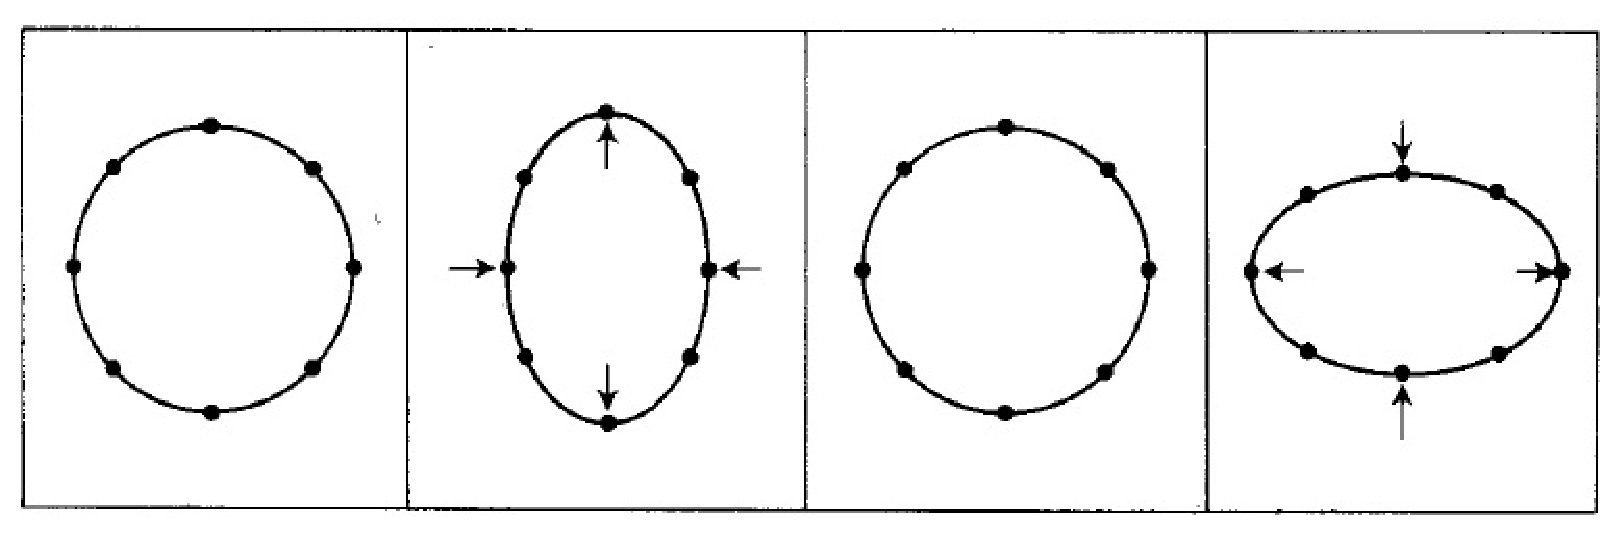
\includegraphics[width=0.5\linewidth]{figures/Introduction/pluspol.eps}
  \caption{effect of plus ($+$) polarisation}
  \label{fig:sub1}
\end{subfigure}\\
\begin{subfigure}{\textwidth}
  \centering
  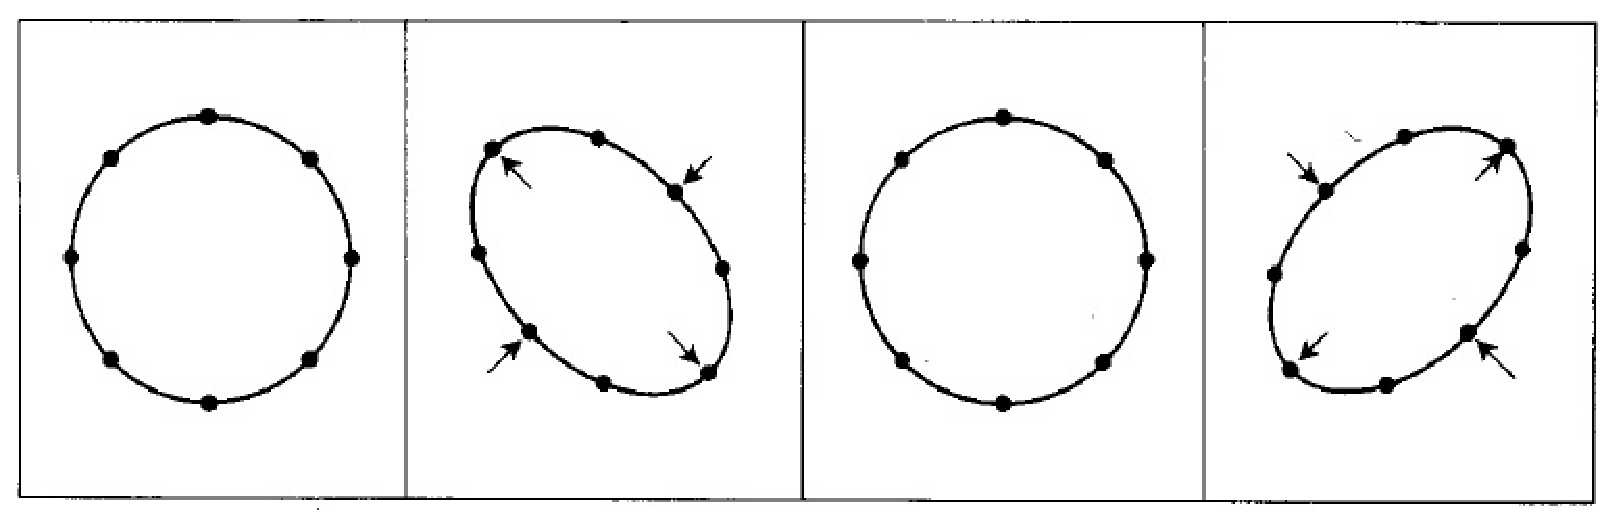
\includegraphics[width=0.5\linewidth]{figures/Introduction/crosspol.eps}
  \caption{effect of cross ($\times$) polarisation}
  \label{fig:sub2}
\end{subfigure}
\caption{Time sequence showing the effect of an oscillatory linear plane GW with (a) plus and (b) cross polarisation.}
\label{fig:Polarisation}
\end{figure}


\section{Compact Binary Mergers}

A binary system with compact objects such as black holes or neutron stars which are sufficiently close together will emit energy via the gravitational radiation. As the system evolves in frequency the radiated energy increases and the compact objects in-spiral each other. 
These are currently the most commonly detected sources of gravitational waves. 

\subsection{Modeling compact binary mergers}

A compact binary merger involves two massive objects in a close orbit, spiraling inwards due to the emission of gravitational waves, until they eventually merge. The signal from such an event can be characterized by various parameters, including the masses and spins of the two objects, the distance to the source, the inclination of the orbital plane relative to the observer, and the sky location of the source.


Different Binaries and Mathematical Formalisms:
Binary Black Holes (BBH): BBH mergers involve two black holes spiraling inwards and merging. The post-Newtonian formalism, which provides a series expansion in terms of the velocity of the objects divided by the speed of light, can be used to describe the inspiral phase. For the merger and ringdown phases, numerical relativity simulations are required, as the gravitational fields are extremely strong and the dynamics are highly nonlinear.

Binary Neutron Stars (BNS): BNS mergers involve two neutron stars. In addition to the gravitational wave emission, these events can also result in electromagnetic signals, such as gamma-ray bursts. The inspiral can be modeled using post-Newtonian formalism, but tidal effects (which are important for neutron stars) must also be taken into account. Numerical relativity simulations are required to accurately model the merger and post-merger phases, including the potential formation of a hypermassive neutron star or a black hole.

Neutron Star – Black Hole Binaries (NSBH): These binaries involve a neutron star and a black hole. The modeling of these systems is similar to BNS mergers, but with additional complexity due to the interaction of the neutron star with the black hole’s tidal field, which can lead to the disruption of the neutron star.

\subsection{Orbital mechanics and the Post Newtonian treatment}

Gravitational waves are generated by the change in the quadrupolar moment which can occur for sources that are broadly classified in four different types. \\

\begin{itemize}
\item Continuous Gravitational Waves
\item Stochastic Gravitational Wave Background
\item Supernovae
\item Primordial Gravitational Waves
\end{itemize}


\subsection{Gravitational waveforms}

Gravitational waves can be modeled by numerically solving the Einstein equations. 

A gravitational wave signal from a compact binary merger can be divided into three main parts:
Inspiral: The phase where the two objects are orbiting each other, gradually coming closer. The waveform in this phase can be approximated using post-Newtonian theory or effective-one-body formalism.

Merger: The phase where the two objects coalesce. PN approximations begin breaking down as these objects come closer. Analytical approximations are no longer valid and thus, this phase requires numerical relativity simulations for accurate modeling.

Ringdown: The phase after the merger, where the newly formed object (a black hole or a neutron star) settles into its final state, emitting gravitational waves in the process. The ringdown can be modeled using black hole perturbation theory, specifically quasi-normal modes.

Various waveform models have been proposed and developed to describe the full signal from compact binary mergers, combining analytical and numerical techniques. These include:

Phenomenological Models: These models use analytical fits to numerical relativity simulations to describe the entire waveform. Phenomenological models for gravitational waves from coalescing binary systems (such as binary black holes or neutron stars) are crucial for the detection and interpretation of gravitational wave signals. These models aim to provide accurate and computationally efficient descriptions of the signals across all phases of the coalescence: inspiral, merger, and ringdown. Below, I will delineate the construction of phenomenological waveform models, highlighting the key steps and methodologies involved.

1. Inspiraling Phase: Post-Newtonian Theory
    Post-Newtonian Expansion: The inspiral phase, where the binary components are far apart and moving slowly compared to the speed of light, is modeled using post-Newtonian (PN) theory. This involves expanding the equations of motion and gravitational waveforms in powers of $v/c$ (velocity of the bodies divided by the speed of light).

    Incorporating Spin Effects: The effects of the spins of the binary components are included using spin-orbit and spin-spin coupling terms in the post-Newtonian expansion.

    Higher-Order Corrections: The accuracy of the model is improved by including higher-order PN terms. The coefficients of these terms are calculated analytically or fitted to numerical relativity simulations.

2. Merger Phase: Numerical Relativity
    Numerical Simulations: The merger phase, where the binary components are in close proximity and moving at a significant fraction of the speed of light, requires numerical relativity simulations to accurately model. These simulations involve solving Einstein’s equations directly on a computer grid.

    Fitting to Numerical Data: The parameters of the phenomenological model are tuned to provide the best match to the numerical relativity waveforms. This process may involve fitting formulae that describe how the waveform changes with different binary parameters (such as masses and spins).

3. Ringdown Phase: Black Hole Perturbation Theory
    Quasi-Normal Modes: After the merger, the resulting single black hole undergoes a ringdown phase, emitting gravitational waves as it settles to a stable state. This phase is modeled using black hole perturbation theory, identifying the quasi-normal modes of the final black hole.

    Matching to Merger: The ringdown waveform is matched onto the end of the merger waveform, ensuring a smooth transition between the two phases.

Creating a Complete Model
    Matching Across Phases: The inspiral, merger, and ringdown phases are combined to create a complete waveform model. This requires careful matching of the waveforms at the boundaries between the phases to ensure consistency and accuracy.

    Parameterization: The complete model is parameterized in terms of the physical parameters of the binary system, such as the component masses, spins, and orbital parameters. This allows for rapid generation of waveforms for different binary configurations.

5. Validation and Calibration
    Comparison to Numerical Relativity: The phenomenological model is validated by comparing its predictions to a wide range of numerical relativity waveforms, ensuring accuracy across the parameter space.

    Calibration: The model may be calibrated to improve agreement with numerical relativity simulations, particularly in regions of the parameter space where the post-Newtonian or perturbative approximations are less accurate.

6. Application in Data Analysis
    Rapid Waveform Generation: The phenomenological model allows for the rapid generation of waveforms, which is essential for gravitational wave data analysis, including signal detection and parameter estimation.
    
    Coverage of Parameter Space: The model is designed to accurately cover the entire parameter space of binary coalescences, allowing for the analysis of a wide range of binary systems.


Effective-One-Body (EOB) Models: These models map the two-body problem onto an effective one-body problem, using results from post-Newtonian theory and numerical relativity. It was initially developed to overcome the limitations of post-Newtonian theory in the highly relativistic regime of binary mergers. 

1. Conceptual Foundation

The EOB method transforms the problem of two interacting bodies in a binary system into an equivalent problem of a single test particle moving in an effective external gravitational field. This effective field encapsulates the complex interactions between the two bodies. The transformation simplifies the problem, making it more tractable, especially in the strong-field, fast-motion regime close to merger.

2. Mapping to an Effective Problem
    Effective Metric: An effective metric is introduced to describe the gravitational field in which the test particle moves. This metric is parameterized in terms of the masses and spins of the binary components.

    Reduced Mass and Total Mass: The dynamics are described in terms of the reduced mass $\mu=\dfrac{m_1m_2}{m_1+m_2}$ and the total mass $M=m_1+m_2$, where $m_1$ and $m_2$ are the masses of the two bodies.

    Hamiltonian: An effective Hamiltonian is constructed to describe the motion of the test particle. This Hamiltonian includes not only the leading-order (Newtonian) terms but also higher-order post-Newtonian corrections and resummed terms that capture strong-field effects.

3. Resumming Post-Newtonian Terms
    Padé Approximants: The post-Newtonian series is resummed using techniques like Padé approximants to improve its convergence and extend its validity into the strong-field regime.

    Resummation of the Energy Flux: The energy flux of gravitational waves emitted by the system is also resummed to improve its behavior in the strong-field, fast-motion regime.

4. Calibration to Numerical Relativity
    Tuning Free Parameters: The EOB model includes several free parameters that cannot be determined purely analytically. These parameters are calibrated by comparing EOB predictions to fully numerical solutions of Einstein’s equations for binary systems, obtained via numerical relativity simulations.

    Improving the Model: The calibration process helps in refining the EOB model, ensuring that it accurately captures the complex dynamics of binary coalescence, especially during the merger and ringdown phases.

5. Waveform Generation
    Generating Inspirals: The EOB approach generates waveforms for the inspiral phase of the binary coalescence, capturing the increasing amplitude and frequency of the gravitational waves as the bodies spiral together.

    Extending to Merger and Ringdown: By incorporating information from numerical relativity, the EOB model is extended to accurately describe the merger of the two bodies and the ringdown of the resulting single compact object.

6. Application in Gravitational Wave Astronomy
    Parameter Estimation: EOB models are crucial for interpreting gravitational-wave signals detected by observatories like LIGO and Virgo, allowing for the extraction of physical parameters of the binary system.

    Real-time Data Analysis: Due to their efficiency in generating waveforms, EOB models are particularly useful for real-time data analysis and rapid characterization of gravitational-wave events.

7. Continuous Development and Validation
    Incorporating Spin and Precession: Efforts are ongoing to improve EOB models by incorporating effects like spin-precession and higher-order mode contributions, which are important for accurately modeling systems with spinning and misaligned components.

    Validation Across the Parameter Space: EOB models are continuously validated and updated based on comparisons with new numerical relativity simulations, ensuring their reliability across the vast parameter space of binary configurations.


Hybrid Models: These models combine post-Newtonian or EOB waveforms for the inspiral with NR waveforms for the merger and ringdown.


\section{Formation and evolution mechanisms of binary mergers}

Neutron stars (NS) and black holes (BH) with stellar masses typically emerge from the end stages of massive stars. These massive stars are usually not solitary; they often exist in pairs or even more complex groups, with many engaging in interactions with their companions, as illustrated in the works of Sana et al. (2012) and Moe and Di Stefano (2017). The dynamics of these interactions, which significantly shape the destiny and observable traits of the stars—as well as the events they catalyze, like double compact object (DCO) mergers—are not fully understood .

Gravitational wave (GW) detections offer a promising avenue for unveiling the intricate mechanisms governing the life cycles of these massive stellar entities. Yet, when such NS or BH formations are situated in regions bustling with stellar activity, the frequent stellar run-ins can modify their characteristics significantly. Under these circumstances, repeated mergers are a possibility, hinting that some GW events we observe may involve BHs that are not straightforwardly linked to the immediate outcomes of stellar or binary evolution.

One of the primary complexities in the field of GW astrophysics is the ambiguity in interpreting observational data, which can vary based on the postulated history of the merger's formation . Therefore, distinguishing the unique origins of merger events based on their observational signatures is of paramount importance.

An illustrative example is provided by the most massive GW event on record to date (GW190521), which was interpreted as a merger between two BHs with a combined mass of 150 $M_{\odot}$, with the primary BH weighing over 65 $M_{\odot}$ at a 99\% confidence level (refer to Abbott et al. 2020b,c, and see also Fishbach and Holz 2020 for a perspective that a mass over 120 $M_{\odot}$ is plausible). The formation of such a massive BH through isolated binary evolution is deemed highly improbable, as it would typically be in the range of 50 $M_{\odot}$ to 120 $M_{\odot}$ — a region expected to yield no remnant due to pair-instability supernovae (PISN), according to predictions by Bond et al. (1984) and Woosley and Heger (2006). Should GW190521 indeed include a BH mass within this predicted gap, it would strongly suggest an origin outside of isolated binary star evolution.

However, drawing broader conclusions about the evolution of massive stars from singular observations requires an understanding of how typical such instances are. As the pool of GW data grows, it allows for a more detailed understanding of the properties of local DCO mergers, such as the rates at which they occur and their mass distributions. Weaker constraints exist on their spin distributions and sky localizations, which could indicate potential host galaxies.

One particularly interesting discovery is that the bulk of the BHBH mergers observed—32 out of 44 systems—feature at least one BH exceeding 30 $M_{\odot}$ in mass. The prevalence of such massive BHs among GW findings, while anticipated due to selection biases (discussed in Sec. 1.1.2), is noteworthy since electromagnetically observed systems with BHs before the era of GW detection were estimated to be less than 20 $M_{\odot}$ (e.g., Tetarenko et al., 2016; Miller-Jones et al., 2021). The maximum mass achievable by a BH from stellar origin is understood to be metallicity-dependent, with wind mass loss rates during the massive star phase increasing with metal content, thus reducing the final mass of the BH (Vink et al. 2001; Vink and de Koter 2005). This has led to theories that the massive BHBH mergers detected through GWs may arise from low-metallicity star formation regions or potentially from previous merger events.

The potential for gravitational wave data to reveal discontinuities, such as mass gaps or cutoffs, within the compact object mass spectrum is of significant interest for its implications on core collapse and stellar explosion physics. Differing explosion models predict varying outcomes, such as a mass gap between approximately 3 - 5 $M_{\odot}$ due to the dynamics of massive stellar core collapse, with others anticipating a more uniform distribution (for instance, see Fryer et al., 2012). GW data can thus provide valuable constraints on these theoretical models.

The advancement in detector sensitivity is starting to allow examination of the BHBH population across cosmic time. The anticipated evolution of GW detector capabilities, with projects like Cosmic Explorer and Einstein Telescope (outlined by Reitze et al. 2019 and Maggiore et al. 2020), promises to map this dependency across the span of cosmic star formation history. Such insights could enhance our comprehension of the Universe's chemical evolution and its correlation with unresolved questions. This chapter will provide a comprehensive overview of these formation and evolution mechanisms.

\textbf{Formation channels}

\textbullet{Primordial Formation}

Some compact binaries are believed to form directly from the primordial gas in the early Universe. These binaries originate from density fluctuations in the early Universe, leading to the formation of closely-packed binaries.

\textbullet{Tidal Capture}

In dense stellar environments like globular clusters, stars can come close enough for tidal forces to dissipate energy and form a bound pair. Over time, through dynamical interactions and gravitational radiation, these pairs can evolve into compact binaries.

\textbf{Evolutionary Pathways}

\textbullet{Common Envelope Phase}

One of the most significant phases in the evolution of compact binary systems is the common envelope (CE) phase. This occurs when one of the stars in the binary expands, engulfing its companion. Drag forces within the envelope can cause the companion to spiral inward, leading to a closer binary system. If enough energy is released, the envelope can be ejected, leaving behind a compact binary.

\textbullet{Mass Transfer}

After the CE phase or in the absence of it, one star can transfer mass to its companion. Depending on the mass ratio and other properties, this mass transfer can be stable or unstable, leading to different outcomes:

    Roche Lobe Overflow (RLOF): When a star fills its Roche lobe, the outer layers can be transferred to its companion. This process can lead to drastic changes in the binary configuration.

    Thermal Timescale Mass Transfer: In cases where the mass-losing star is much more massive than its companion, the mass transfer can be rapid, leading to the formation of a helium core.

\textbullet{Stellar Collisions}

In dense stellar environments, direct collisions between stars can lead to the formation of compact binaries. These collisions can merge two stars or strip the outer layers of one, leaving behind a compact remnant.

\textbullet{Gravitational Radiation}

Compact binaries, especially those involving neutron stars or black holes, can emit gravitational waves. This radiation causes the binary to lose energy, leading to a decrease in the orbital separation and eventually merger.

\textbf{End Stages}

\textbullet{Supernova Explosions}

If one component of the binary undergoes a supernova explosion, it can disrupt the binary. Alternatively, if the binary remains bound, the system may evolve into a compact binary with a neutron star or a black hole.

\textbullet{Mergers}

When the separation between binary components decreases to a critical value, the binary can merge, leading to various outcomes:

    White Dwarf Mergers: Can lead to a type Ia supernova.

    Neutron Star Mergers: Result in the emission of intense gravitational waves and can form a black hole.

    Black Hole Mergers: Produce powerful gravitational waves detectable by observatories like LIGO and Virgo.







\chapter{Data analysis for gravitational wave from compact binary mergers}

The current operational gravitational wave observatories include the Laser Interferometer Gravitational-Wave Observatory (LIGO), with its two detectors in Hanford, Washington, and Livingston, Louisiana, in the United States; Virgo, located near Pisa, Italy; and KAGRA, in Japan. These detectors are part of a growing global network that collaborates to triangulate the source of gravitational waves and improve the sensitivity of detections.

The LIGO observatories in Hanford and Livingston are identical in their L-shaped design, with each arm being 4 kilometers long. They use laser interferometry to measure the minute distortions in spacetime caused by passing gravitational waves. The arms are kept in a near-perfect vacuum to minimize disturbances, and mirrors at the ends of each arm are suspended to isolate them from external vibrations. Virgo is a gravitational wave detector that features a 3-kilometer-long L-shaped interferometer. While slightly shorter than the LIGO arms, Virgo's design has incorporated advanced technology for noise reduction and has made significant contributions to the global detection efforts. KAGRA is unique among the gravitational wave detectors as it is located underground in the Kamioka mine, which helps to shield it from seismic noise and provides a stable thermal environment. KAGRA uses a 3-kilometer-long L-shaped interferometer like Virgo and is designed to operate at cryogenic temperatures to reduce thermal noise.


\section{Data from the ground based interferometers}
The primary data is the ``strain" measured in the interferometer's arms, which is a dimensionless measure of the fractional change in length that one of the interferometer's arms experiences relative to the other: a gravitational wave passing through the interferometer will stretch one arm and compress the other. It is represented by the symbol $h$, and it's calculated by the change in length ($\delta L$) divided by the original length of the interferometer’s arm ($L$): $h = \delta L / L$. This strain is incredibly small—on the order of $10^-{21}$, meaning the instruments need to detect changes in length smaller than one-thousandth of a proton diameter.
\subsection{Noise sources}

To achieve the extraordinary sensitivity means that these detectors must deal with a plethora of noise sources that can mask or mimic gravitational wave signals. Below is an expanded look at the main types of noise that affect ground based gravitational wave observatories:

Quantum noise in gravitational wave detectors arises from the Heisenberg uncertainty principle, which limits the precision with which pairs of physical properties, like position and momentum, can be known.
\begin{itemize}
    \item Shot Noise: This is a form of quantum noise that arises because light consists of discrete particles (photons). When measuring the interference pattern in an interferometer, the discrete arrival of photons causes statistical fluctuations in the detected light intensity. At high laser power, shot noise predominates and limits the high-frequency sensitivity of the detectors.
    \item Radiation Pressure Noise: At lower frequencies, the variability is dominated by radiation pressure noise. This is the fluctuation in force exerted by photons as they bounce off the mirrors. It introduces a quantum limit to the low-frequency sensitivity due to the momentum transfer of the light.
\end{itemize}


Thermal noise is related to the random motion of atoms and molecules:
\begin{itemize}
    \item Suspension Thermal Noise: The motion of the suspension fibers can introduce noise due to thermal vibrations. Advanced detectors use materials such as fused silica with very low mechanical losses to suspend the mirrors, minimizing this source of noise.
    \item Mirror Thermal Noise: The mirrors themselves are also sources of thermal noise. Brownian motion within the reflective coating and the substrate material of the mirrors can lead to fluctuations in the reflected light phase. Lowering temperatures (as with KAGRA) can reduce such noise.
\end{itemize}

Seismic noise is the result of ground vibrations transmitted through the Earth, originating from natural and anthropogenic sources:

\begin{itemize}
    \item Ground Vibrations: These are the primary source of noise below a few tens of hertz. They can be caused by earthquakes, ocean waves, or even nearby human activity such as traffic or industrial work.
    \item Isolation Techniques: Advanced isolation systems are used to minimize this noise, including active seismic isolation, which uses sensors to detect ground motion and actuators to counteract it, and passive isolation, such as layers of springs and masses that absorb vibrations.
\end{itemize}

Gravity gradient noise, also known as Newtonian noise, is due to fluctuations in the local gravitational field:
\begin{itemize}
    \item  Environmental Factors: These can be caused by atmospheric pressure changes, density changes in the Earth, or even human activity, all of which can create varying gravitational forces on the detector components.
    \item Subtraction Techniques: This type of noise is particularly challenging to mitigate because it cannot be shielded against in the same way as electromagnetic noise. Efforts to subtract it involve modeling the environmental effects and removing their signature from the data.
\end{itemize}

Instrumental noise arises from the detector's components:
\begin{itemize}
    \item  Electronic Noise: In the photodetectors and other electronic systems, inherent noise can be introduced. This is typically white noise that can be well-characterized and filtered.
    \item Calibration Errors: Uncertainty in the detector's response to gravitational waves can also introduce noise into the measurement. Regular calibration is necessary to minimize this source.
\end{itemize}

\begin{figure*}
    \centering
    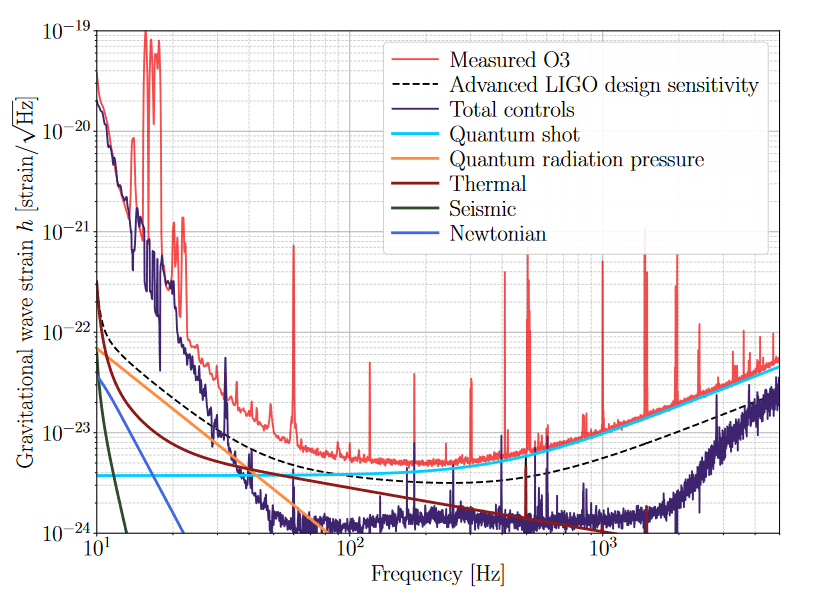
\includegraphics[width=\textwidth]{figures/basic_data_analysis/O3_noise_budget.PNG}
    \caption{O3 noise budget. Only few noise sources are shown for a simplified picture. \cite{aLIGO:2020wna}}
    \label{fig:O3_noise_budget}
\end{figure*}







\subsection{Basics of Fourier domain analysis}

Fourier domain analysis is a mathematical technique widely used in the field of data analysis to extract signal information from noisy data. Gravitational wave signals are often buried in noise, making it difficult to detect them in the time domain. However, by transforming the data into the frequency domain using Fourier analysis, it becomes easier to identify and analyze these signals.


Suppose we have a function of time $x(t)$. Let us denote the Fourier transform of $x(t)$ by $\tilde{x}(f)$, which is given by
    \begin{align}
        \tilde{x}(f) = \int_{-\infty}^{\infty} e^{-2\pi i ft} x(t) dt,
    \end{align}
    similarly, the inverse Fourier transform is given by
    \begin{align}
        x(t) = \int_{-\infty}^{\infty} e^{2\pi i f t} \tilde{x}(f) df.
    \end{align}

Write the discretized form of Fourier transform and talk about the Nyquist-frequency

\subsection{Modeling and measuring the noise}
The noise time series in a detector like LIGO is a complex superposition of various stochastic processes and we represent this time series $n(t)$ which can be considered as a vector $\textbf{n}$ (or random process). Each of the discrete samples $n_i = n(t_i)$ is described as random variable with values according a probability distribution $p_i = p(n_i)$, and the complete noise vector is then associated to to a joint probability distribution $p(\textbf{n})$. 

Features of the shape of a probability distribution can be captured by measuring moments. The first two moments of a stochastic process are often of particular interest -- mean $\mu = \langle \textbf{n}\rangle$ and covariance $C_{ij} = \langle(n-\mu_{i})(\mu_{j}-n)\rangle$, where $\langle\rangle$ is defined as the expectation value of a random variable over time. Assuming the noise process to be \textit{stationary random process} -- the statistical properties do not change over time. The ensemble average is equivalent to a long time average. We can estimate these two quantities from the data with $N$ data samples
\begin{align}
    \mu = \dfrac{1}{N}\sum_{i=1}^{N}n_{i}.
    \label{eq:mean-noise-series}
\end{align}
And, the covariance matrix can be estimated using
\begin{align}
    C_{ij} = (n_{i} - \mu)(\mu - n_j).
    \label{eq:covariance-noise-series}
\end{align}
We can write the joint probabilty distribution of noise $p(\textbf{n})$ in terms of the mean and the covariance matrix which follows a multi-variate normal distribution
\begin{align}
    p(\textbf{n}) = \dfrac{1}{\text{det}(2\pi \textbf{C})^{1/2}}\text{exp}\Bigg[-\dfrac{1}{2} \sum_{ij}(n_{i} - \mu)(\mu - n_j) C_{ij}^{-1} \Bigg],
    \label{eq:joint-pdf-noise}
\end{align}
where $C_{ij}^{-1}$ represents the inverse and $\det{C}$ the determinant of the covariance matrix.


\section{Optimal method to extract signal out of noise: Matched filtering}
At the heart of modeled approaches to detecting compact binary coalescence (CBC) signals lies the matched-filtering method. This technique scans through data from interferometers to identify patterns that match the predicted gravitational wave (GW) signal waveforms referenced in the literature. This section provides a succinct overview of matched filtering and highlights some innovative approaches to enhance the efficiency of these algorithms. Additionally, we reflect on past strategies that have aimed at optimizing matched filtering, as discussed in Section II B.

When it comes to GW signals emanating from CBC sources with circular orbits, they are described by 15 distinct parameters, as cited in studies. These parameters fall into two groups: (1) intrinsic parameters, which include the masses $(m_1, m_2)$ and three-dimensional spin vectors $(\chi_1, \chi_2)$, and (2) extrinsic parameters that are defined from the perspective of the observer—these are the standard spherical coordinates $(D, i, \psi)$, position in the sky $(\theta, \phi)$, and the coalescence timing and phase $(t_c; \phi_c)$. These parameters allow for the GW signal to be precisely depicted through a combination of analytical and numerical methods .

To detect the anticipated GW signal, denoted as $\tilde{h}(f)$ and commonly referred to as the template, one executes matched filtering in the frequency domain. This process assesses the probability that a set of data includes the specific template. The statistic used in matched filtering is essentially a correlation — it involves the Fourier-transformed data $[\tilde{s}(f)]$ and the template $[\tilde{h}(f)]$ — and takes into account the noise power spectral density (PSD) $S_n(f)$. It is established that the matched filter serves as the optimal statistical measure for signal detection amidst stationary Gaussian noise.

The mathematical expression for the complex matched filter statistic is:
\begin{align}
    \label{Eq:matched_filter}
    \braket{s|h} = 4\int_{0}^{\infty} \dfrac{\tilde{s}(f)\tilde{h}^*(f)}{S_n(f)}.
\end{align}
The signal-to-noise (SNR) ratio $\rho$ which is the matched-filter output maximised over an overall amplitude,   
\begin{align}
    \label{Eq:SNR_def}
    \rho^2 = \dfrac{(\Real[\braket{s|h}])^2}{\braket{h|h}}.
\end{align}

Since the signal parameters are unknown, the SNR is maximised over the parameter space. A naive maximisation procedure over the complete 15-dimensional parameter space is computationally challenging. Therefore, the component spins are typically assumed to be aligned with the orbital angular momentum and a search is conducted only for the dominant gravitational-wave mode. Under these assumptions the two polarizations of the signal are related by a simple phase shift $\tilde{h}_+(f) = i \tilde{h}_{\times}(f)$. Using Eqs.(\ref{Eq:Detector_response}) and (\ref{Eq:spherical_harmonics}) the signal seen by the detector in Fourier domain is simplified to 
\begin{align}
    \label{Eq:maxmising_templates}
    \tilde{h}(f) = A(f)e^{i \phi_0}\tilde{h}_0(\kappa; f)e^{2\pi i f t_c},
\end{align}
where $\tilde{h}_0(\kappa)$ depends only on the intrinsic parameters and the extrinsic parameters are factored out as the nuisance parameters -- an overall amplitude $A$ and phase $\phi_0$. 

As per Eq. (\ref{Eq:maxmising_templates}) the SNR is maximised in three categories of parameters -- 1) Intrisinc parameters $\kappa$, 2) fiducial parameters $A$ and $\phi_0$ 3) time of arrival $t_c$. The intrinsic parameters are searched by using a set of discrete points laid out on the four dimensional parameter space $\kappa^{||} = (m_1, m_2, \chi_{1z}, \chi_{2z})$. Waveforms evaluated with parameter values at a given sampled point is referred as templates and together they make up a template bank. The matched filter is repeatedly computed over all the templates to find the best matching template with highest SNR. Simultaneously, for each template, the SNR is maximised over the extrinsic parameters $(D, i, \psi, \alpha, \delta, \varphi_c)$ via the nuisance parameters ($A, \phi_0$) -- first by normalizing the matched filter with the power of the signal $\braket{h|h}$, and then using a quadrature of the SNR to maximise the unknown phase $\phi_0$. The maximization over these nuisance parameters is written as 
\begin{align}
    \mathop{\max}_{\phi_{0}}(\rho^2) = \dfrac{1}{2}\norm{\braket{s|\hat{h}_0}}^2,
    \label{Eq:simplified_statistics}
\end{align}
where $\hat{h}_0 = \tilde{h}_0/\braket{\tilde{h}_0|\tilde{h}_0}^{1/2}$. Finally, the position of the signal is efficiently searched over by performing an inverse fast Fourier transformation (FFT) to obtain the SNR time-series.

\section{Detection in non-Gaussian noise}

\section{}

\chapter{Observations using the PyCBC modeled search pipeline}


In this chapter, I will discuss the PyCBC modeled search pipeline which is primarily designed for detecting and analyzing signals from merging binary systems of compact objects like black holes and neutron stars. It is one of the three major search pipelines that are used to create catalogs of binary merger observations. Since the inception, this pipeline has detected $\sim$ 100 binary mergers. The PyCBC pipeline is highly modular, allowing researchers to adapt its components for different types of analyses. This includes the ability to search for different types of gravitational wave sources, handle various noise artifacts in the detector data, and perform statistical analyses to assess the significance of potential detections.

We will also discuss the gravitational wave catalogs produced using this pipeline as an independent analysis to the LVK results: these were the third (3OGC) and the fourth (4OGC) open gravitational wave catalogs. 

PyCBC is an open-source software package, which allows for collaborative development and improvement by the scientific community. This openness not only fosters transparency in the data analysis methods used in gravitational wave astronomy but also encourages the adoption and adaptation of these techniques in other fields of physics and astronomy.

\section{Description of the PyCBC search pipeline}

\subsubsection{Inputs to the search pipeline}
There are two major inputs to the search pipeline -- 1) GW strain data from one or more detectors and 2) bank of templates corresponding to binary systems that we are searching for. We begin with strain data from the GW observatories typically sampled at a uniform sampling rate of 4098 Hz. This data contains glitches or noise artefacts based on the information provided by a specific auxillary channel. The quality of a data segment is characterized by a data quality flag. Some of the relevant flags are described below:
\begin{enumerate}
    \item DATA: Indicates unavailability of LIGO or Virgo data.
    \item CAT1: Signifies a critical issue with a detector component, leading to major known problems. CAT1 failures are consistent across data analysis groups and such data is not openly accessible.
    \item CAT2: Represents known physical interferences, like high seismic activity, affecting the gravitational wave channel.
    \item CAT3: Indicates unexplained statistical interferences in the gravitational wave channel.
\end{enumerate}

Data-quality investigations might fail to remove all the noise transients. Usually short duration loud transients of order of 1s having SNR $\sim (100--1000)$ can creep in the data. These transients can severely affect the sensitivity of the search by creating large number of spurious triggers. A procedure called \textit{gating} is used to mask the corrupted data around the glitch and to reduce the noise background by removing the spurious noise triggers. 

The second input to the search is the template bank. As described in [], the template bank consists of discrete sets of points over the intrinsic parameters of GW sources. A search for aligned-spin quasi-circular systems typically uses four parameters in a template bank -- detector frame component masses $m_{1}^{det}, m_{2}^{det}$ and component spins $s_{1z}, s_{2z}$. In case of searches for eccentric or precessing sources, additional parameters needs to be incorporated. 

The creation of a template bank entails strategically choosing discrete points within the parameter space. This ensures that any point within the permissible region is within a maximum distance, $ d_{\text{max}} $, from a sampled point. This distance is defined by the mismatch in waveform at these points. The mismatch level dictates the template bank's density and requires careful calibration. A higher mismatch value results in fewer templates, potentially reducing signal SNR, while a lower value increases the number of templates, raising computational demands for matched filtering. The challenge lies in optimizing the number of templates while preserving a set minimum match (1 - mismatch). Various techniques for generating a template bank fall into three main categories: geometric lattice-based methods, stochastic placement algorithms, and hybrid approaches.

Sampling the parameter space by computing mismatches between different waveforms require estimation of noise PSD from the data. A single PSD is used that is valid for the entire search duration to create a single template bank for a detector network. The procedure begins by separately estimating PSDs for each detector in the network using the Welch's method. Data segments of 512s is subdivided into several 16s blocks to estimate PSDs in each block -- for each segment 63 PSDs are estimated. Then the median of the several 16s PSDs is computed to average the power spectrum for the corresponding data segment. Noise PSDs from each segments are combined together as a harmonic mean for the given detector. Repeating the previous steps for each detector and finally taking the average PSD over all detector gives the PSD that is used in generating the template bank. 


\subsubsection{Matched Filtering}
At its core, the PyCBC search pipeline employs the matched-filtering technique. The inputs to the pipeline are discrete quantities -- data $s[t_i]$, templates $h[t_i; \zeta]$ described by parameters $\zeta$, and noise PSD $S_n[f_i]$. The data and the templates are transformed to their Fourier-domain equivalents $\tilde{s}[f_i]$ and $\tilde{h}[f_i]$ respectively, using the Fast Fourier Transform (FFT) algorithm in blocks of $T_B = 512$s. The average PSD is estimated for each block using the median method as discussed previously. Computation of FFTWs is implemented via Intel's Math Kernel Libray on computer processing units (CPUs) or via Nvidia's CUDA library on graphical processing units (GPUs), these libraries are efficient in performing FFTWs in several batches in parallel.  


The discrete form of the Fourier-domain matched filtering equation is given by

\begin{align}
    \rho^2[t_j] \equiv \innerprod{s}{h[\zeta]}[t_j] = 4 \Delta f \sum_{k=1}^{(N-1)/2} \dfrac{\tilde{s}[k]\tilde{h}^*[k;\zeta]}{S_n[k]}e^{2i\pi j k/N},
\end{align}

giving us the matched-filter SNR time series $\rho^2[t_j]$ for a template with the parameters $\zeta$. When the SNR is above a fixed threshold (usually $\sim 5$) then a \textit{trigger} is associated to the corresponding timestamp and the triggering template. In each blocks, triggers are clustered in windows of 1s and only the loudest trigger is stored for further follow-up.  

\subsubsection{Signal Consistency Tests}
Add some intro


\textit{1. Mitigating noise artefacts}\\
Data quality checks and gating vetoes remove only the very loud non-Gaussian noise artefacts. Many glitches are still present in the data that contribute to long tails of the SNR distribution which reduces the significance of a real astrophysical event. The chi-squared test is used to distinguish noise triggers from signal triggers which typically requires intensive computation. It demands an extra $p-$ FFT operations for each SNR time series FFT calculation, corresponding to each frequency bin. The PyCBC pipeline, however, only computes the chi-squared test at clustered trigger times in the SNR series, using an optimized frequency integral rather than FFTs. This method is more efficient unless there's poor data quality with many triggers, where FFT is faster.  

\textit{2. Coincidence test}\\
To minimize the number of false alarms, the PyCBC pipeline also ensures that a potential event is detected with consistent parameters across all detectors. This involves a coincidence test on triggers after vetoing glitches. For a two-detector network, signals must be detected in both detectors within a 15 ms window, allowing for travel time and timing errors. Unlike previous searches that used a metric-based coincidence test, the PyCBC pipeline requires exact-match coincidence, meaning the triggers from each detector must have identical template parameters (masses and spins).

The exact-match test is especially useful for complex gravitational waveforms, like those from spinning neutron stars or black holes, or high-mass waveforms where stochastic templates are used. This method has shown a noticeable improvement in search sensitivity. Triggers passing this test are considered coincident events and are ranked based on a ranking statistic, which is discussed next.

\subsubsection{Ranking the candidates}


\begin{figure}
    \centering
    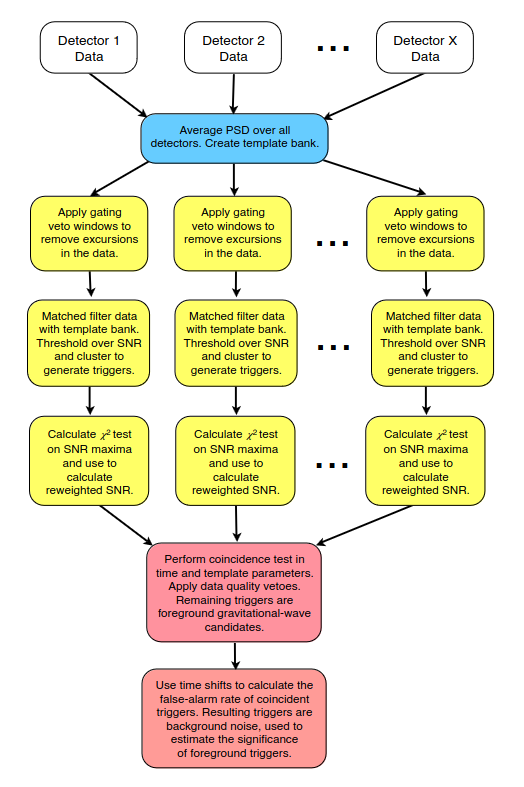
\includegraphics[width=0.75\linewidth]{search_workflow.png}
    \caption{Workflow of the PyCBC search pipeline}
    \label{fig:pycbc_search_workflow}
\end{figure}




\section{Sensitivity of a search}


\section{Current observations of gravitational wave events}
\subsection{The 4OGC and 3OGC catalogs}
\subsection{What do we know from current observations?  }


%Since the current advanced LIGO and advanced VIRGO detectors went online 

\chapter{First search for eccentric spinning neutron star binary mergers}

%This chapter summarizes the search performed in the paper \cite{Dhurkunde:2023qoe}. We have targeted a previously unexplored region of the parameter space for search of eccentric binary systems. We did not find any new significant events, but explore upper limits for four different astrophysical models which have a wide range of astrophysical and physical implications.  

This chapter is a full reprint of \cite{Dhurkunde:2023qoe}, with some minor formatting, and an extra figure and a table. In this work we present our search results for eccentric spinning neutron star binaries from the third observing run of Advanced LIGO and Virgo. Using our search results we put state-of-art constraints for various astrophysical models and predict the capability of future observatories to determine the formation histories of compact binaries.  


\section{Introduction}

Gravitational-wave (GW) astronomy is becoming routine; nearly $100$ compact binary mergers have been observed to date \cite{Nitz:2021zwj,LIGOScientific:2021djp,Olsen:2022pin} using the Advanced LIGO  \cite{LIGOScientific:2014pky} and Advanced Virgo \cite{Acernese:2015gua} observatories. These observations have fueled interest in the long-standing question in astrophysics: \textit{how do compact binary systems form and evolve?} One class of models suggests these systems evolve as isolated stars in the field via common envelope \cite{Belczynski:2001uc, Mennekens:2013dja, Chu:2021evh}, stable mass transfer \cite{Klencki:2021hxe,vandenHeuvel:2017pwp} or via chemically homogeneous mixing \cite{Mandel:2015qlu, Marchant:2016wow}. Alternatively, they may be a result of a dynamical encounter of two or more separately evolved compact objects in dense environments such as globular clusters \cite{Vesperini:2010zi,Fragione:2018vty, Rodriguez:2017pec,Sedda:2020wzl}, nuclear star clusters \cite{Fragione:2018yrb, Wang:2020jsx}, young star clusters \cite{Banerjee:2020qub, Santoliquido:2020bry}, or active galactic nuclei \cite{Bartos:2016dgn, Tagawa:2020qll}.
Current GW catalogs suggest that multiple formation pathways contribute to the population of binary black hole (BBH) mergers in the Universe rather than a single preferred channel \cite{Zevin:2020gbd,KAGRA:2021duu}. However, there is an insufficient number of observed neutron star binaries (BNS or NSBH) to determine if there is a preference for a single dominant channel or several competing channels present~\cite{KAGRA:2021duu,Belczynski:2017mqx}.

%observations using GWs \cite{Nitz:2021zwj,LIGOScientific:2021djp,Olsen:2022pin} or radio pulsars \cite{Tauris:2017omb,Ozel:2015fia} 

Each formation channel makes distinct predictions for the distribution of binary properties, e.g. masses, spins, eccentricity and merger rate~\cite{Mandel:2021smh}. Distinguishing these channels could be done by careful comparison of large number of detected events or by identifying rare events with properties that are unique to a specific channel \cite{Zevin:2020gbd,Zevin:2021rtf,Dhurkunde:2022aek}. Orbital eccentricity carries a strong signature of a binary's evolutionary history: although the initial eccentricity of a binary is close to unity due to asymmetrical supernovae kicks  \cite{Hobbs:2005yx, Verbunt:2017zqi}, the evolution of eccentricity is influenced by the binary's surrounding environment.  In field binaries, energy dissipation solely occurs through GW emission, resulting in a swift reduction in eccentricity as the system evolves in frequency -- becoming nearly negligible when GW frequency reaches the sensitive band of current GW observatories (e.g 10 Hz) \cite{Peters:1964zz}. Whereas, in dense environments, angular momentum exchanges with a third compact object via the Lidov-Kozai (LK) mechanism \cite{LIDOV1962719,Kozai:1962zz, Antognini:2015loa} can result in sustained non-negligible eccentricities at GW frequencies sensitive to current detectors. 

\begin{sidewaysfigure}
        \centering
    \includegraphics[width=\textwidth]{figures/ecc_search/eccentricity_dist.png}
    \caption{Distribution of orbital eccentricities (left column) for different formation models \cite{Belczynski:2017mqx, Sedda:2020wzl,Trani:2021tan,Fragione:2018yrb} at the time of formation of compact binaries (green) and when the dominant-mode of GW frequency reach 10 Hz (pink). All four models predict mergers to born with high natal eccentricities. Considering energy loss via GW only, eccentricity is quickly radiated away as evident by the clear shift in the distributions for the isolated BNS channel \cite{Belczynski:2017mqx} and for NSBH mergers in globular clusters \cite{Sedda:2020wzl}. The nuclear cluster \cite{Fragione:2018yrb} and hierarchical triples \cite{Trani:2021tan} models describe eccentricity enhancing scenarios where NSBH binaries can retain non-negligible eccentricities at 10 Hz. We also show the chirp mass distribution predicted by each model in the second column and the estimated chirp masses of the observed BNS (GW170817, GW190425) and NSBH (GW200105, GW200115) events.}
    \label{fig:eccentricity-dist}    
\end{sidewaysfigure}

We highlight four formation scenarios in Fig. \ref{fig:eccentricity-dist} as a fiducial comparison \cite{Belczynski:2017mqx,Sedda:2020wzl,Trani:2021tan,Fragione:2018yrb}. We have considered two models without eccentricity enhancing mechanisms -- one for isolated BNS binaries \cite{Belczynski:2017mqx} and for NSBH systems in globular clusters \cite{Sedda:2020wzl}. We also study two models with eccentricity inducing mechanisms -- NSBH systems in hierarchical triples \cite{Trani:2021tan} and in nuclear clusters \cite{Fragione:2018yrb}. In models influenced by the LK mechanism, up to $80\%$ of the systems could possess eccentricity $e_{10} \geq 0.01$ (eccentricity at dominant-mode gravitational-wave frequency of 10 Hz ($e_{10}$)) \cite{Hamers:2019oeq, Fragione:2018yrb,Trani:2021tan, Silsbee:2016djf,Rodriguez:2018jqu}, and in the absence, only up to $5\%$ of the sources exceed this eccentricity \cite{Sedda:2020wzl, Belczynski:2017mqx}. Observation of an eccentric system would clearly indicate the presence of a dynamical channel. Even a null detection would allow us to put tighter constraints on the predicted merger rates which are highly sensitive to the unconstrained parameters describing physical process such as common-envelope evolution \cite{Marchant:2021hiv,Santoliquido:2020bry, Baibhav:2019gxm}, natal supernovae kicks \cite{Belczynski:2001uc,Hamers:2019oeq,Trani:2021tan,Santoliquido:2020bry,Silsbee:2016djf, Richards:2022fnq, Baibhav:2019gxm} or dynamics of dense environments \cite{Fragione:2018yrb,Ford:2021kcw,Petrovich:2017otm}. 


Four neutron star binary mergers have been observed to date: two BNS mergers GW170817 \cite{LIGOScientific:2017vwq} and GW190425 \cite{LIGOScientific:2020aai} and two potential NSBH mergers GW200105 and GW200115 \cite{LIGOScientific:2021qlt}. All of these binaries were found using searches that only model quasi-circular binary orbits \cite{Messick:2016aqy,Aubin:2020goo,Allen:2005fk,Usman:2015kfa}. If neutron star binaries have sufficiently high eccentricities, they would be missed by these searches \cite{Huerta:2013qb,Lenon:2021zac}.   The two BNS mergers have eccentricities limited to $e_{10} \leq 0.024$ and $e_{10} \leq 0.048$ for GW170817 and GW190425, respectively \cite{Lenon:2020oza}. 
% need somethign more after this sentence
%The measurement of a nonzero eccentricity of a binary merger would be a smoking gun for a dynamical formation channel. 
In this Letter, we report the results for the first search for NSBH and the latest from BNS aligned-spin eccentric systems. A previous search for BNS mergers in the data from Advanced LIGO and Virgo's second observing run used a narrower range of binary masses (shown in Fig. \ref{fig:search_region}) and did not account component-object spins \cite{Nitz:2019spj}. Searches for eccentric subsolar binaries has also been performed \cite{Nitz:2021vqh,Wang:2021qsu}. Only unmodeled searches have been performed for eccentric BBH systems ~\cite{LIGOScientific:2019dag, LIGOScientific:2023lpe, Pal:2023dyg}. While these searches did not yield any new candidates, they constrained the local merger rate to be less than: $1700$ mergers $\text{Gpc}^{-3} \text{Yr}^{-1}$ for BNS systems with $e_{10} \leq 0.43$ and $0.33$ mergers $\text{Gpc}^{-3} \text{Yr}^{-1}$ for BBH systems with total mass $M \in [70M_{\odot},200M_{\odot}]$ and $e_{15} < 0.3$ at 90\% confidence. In addition, radio pulsar surveys have discovered over twenty BNS systems exhibiting a broad range of eccentricities between 0.06 and 0.8 \cite{Bernadich:2023uru} (see Table I). These observations constrain the BNS local merger rate to $293^{+222}_{-103}$ $\text{Gpc}^{-3} \text{Yr}^{-1}$.


We do not find any new mergers in the public data from the third observing run (O3) of Advanced LIGO and Advanced Virgo observatories. We use our observations and the capabilities of future observatories to constrain an isolated BNS model and three different models for NSBH mergers in globular clusters, nuclear clusters and hierarchical triples: our observations restrict the rate of mergers for BNS binaries to be less than $\sim 150$ mergers $\text{Gpc}^{-3}\text{Yr}^{-1}$ and less than $\sim $ 50 -- 100 mergers $\text{Gpc}^{-3}\text{Yr}^{-1}$ for NSBH binaries at 90\% confidence. These constraints assume that the prior observed BNS and NSBH mergers are from alternate formation channels. Assuming they are from one or more of the channels we consider, the measured rate would be consistent given the sparsity of observations. We predict the capabilities of improved second generation and upcoming third-generation GW observatories to use eccentric binary observations to constraint formation models. We find that a network of Cosmic Explorer (CE) (40 km) + CE (20km) observatories will detect the majority of sources from each of these models and could determine that a subset of the population have non-negligible eccentricities. A network of three $\text{A}^{\#}$ observatories would require at least $\sim$ two years of observation to detect a non-negligible eccentric NSBH merger from hierarchical triples or nuclear clusters.    

\begin{figure}
    \centering
    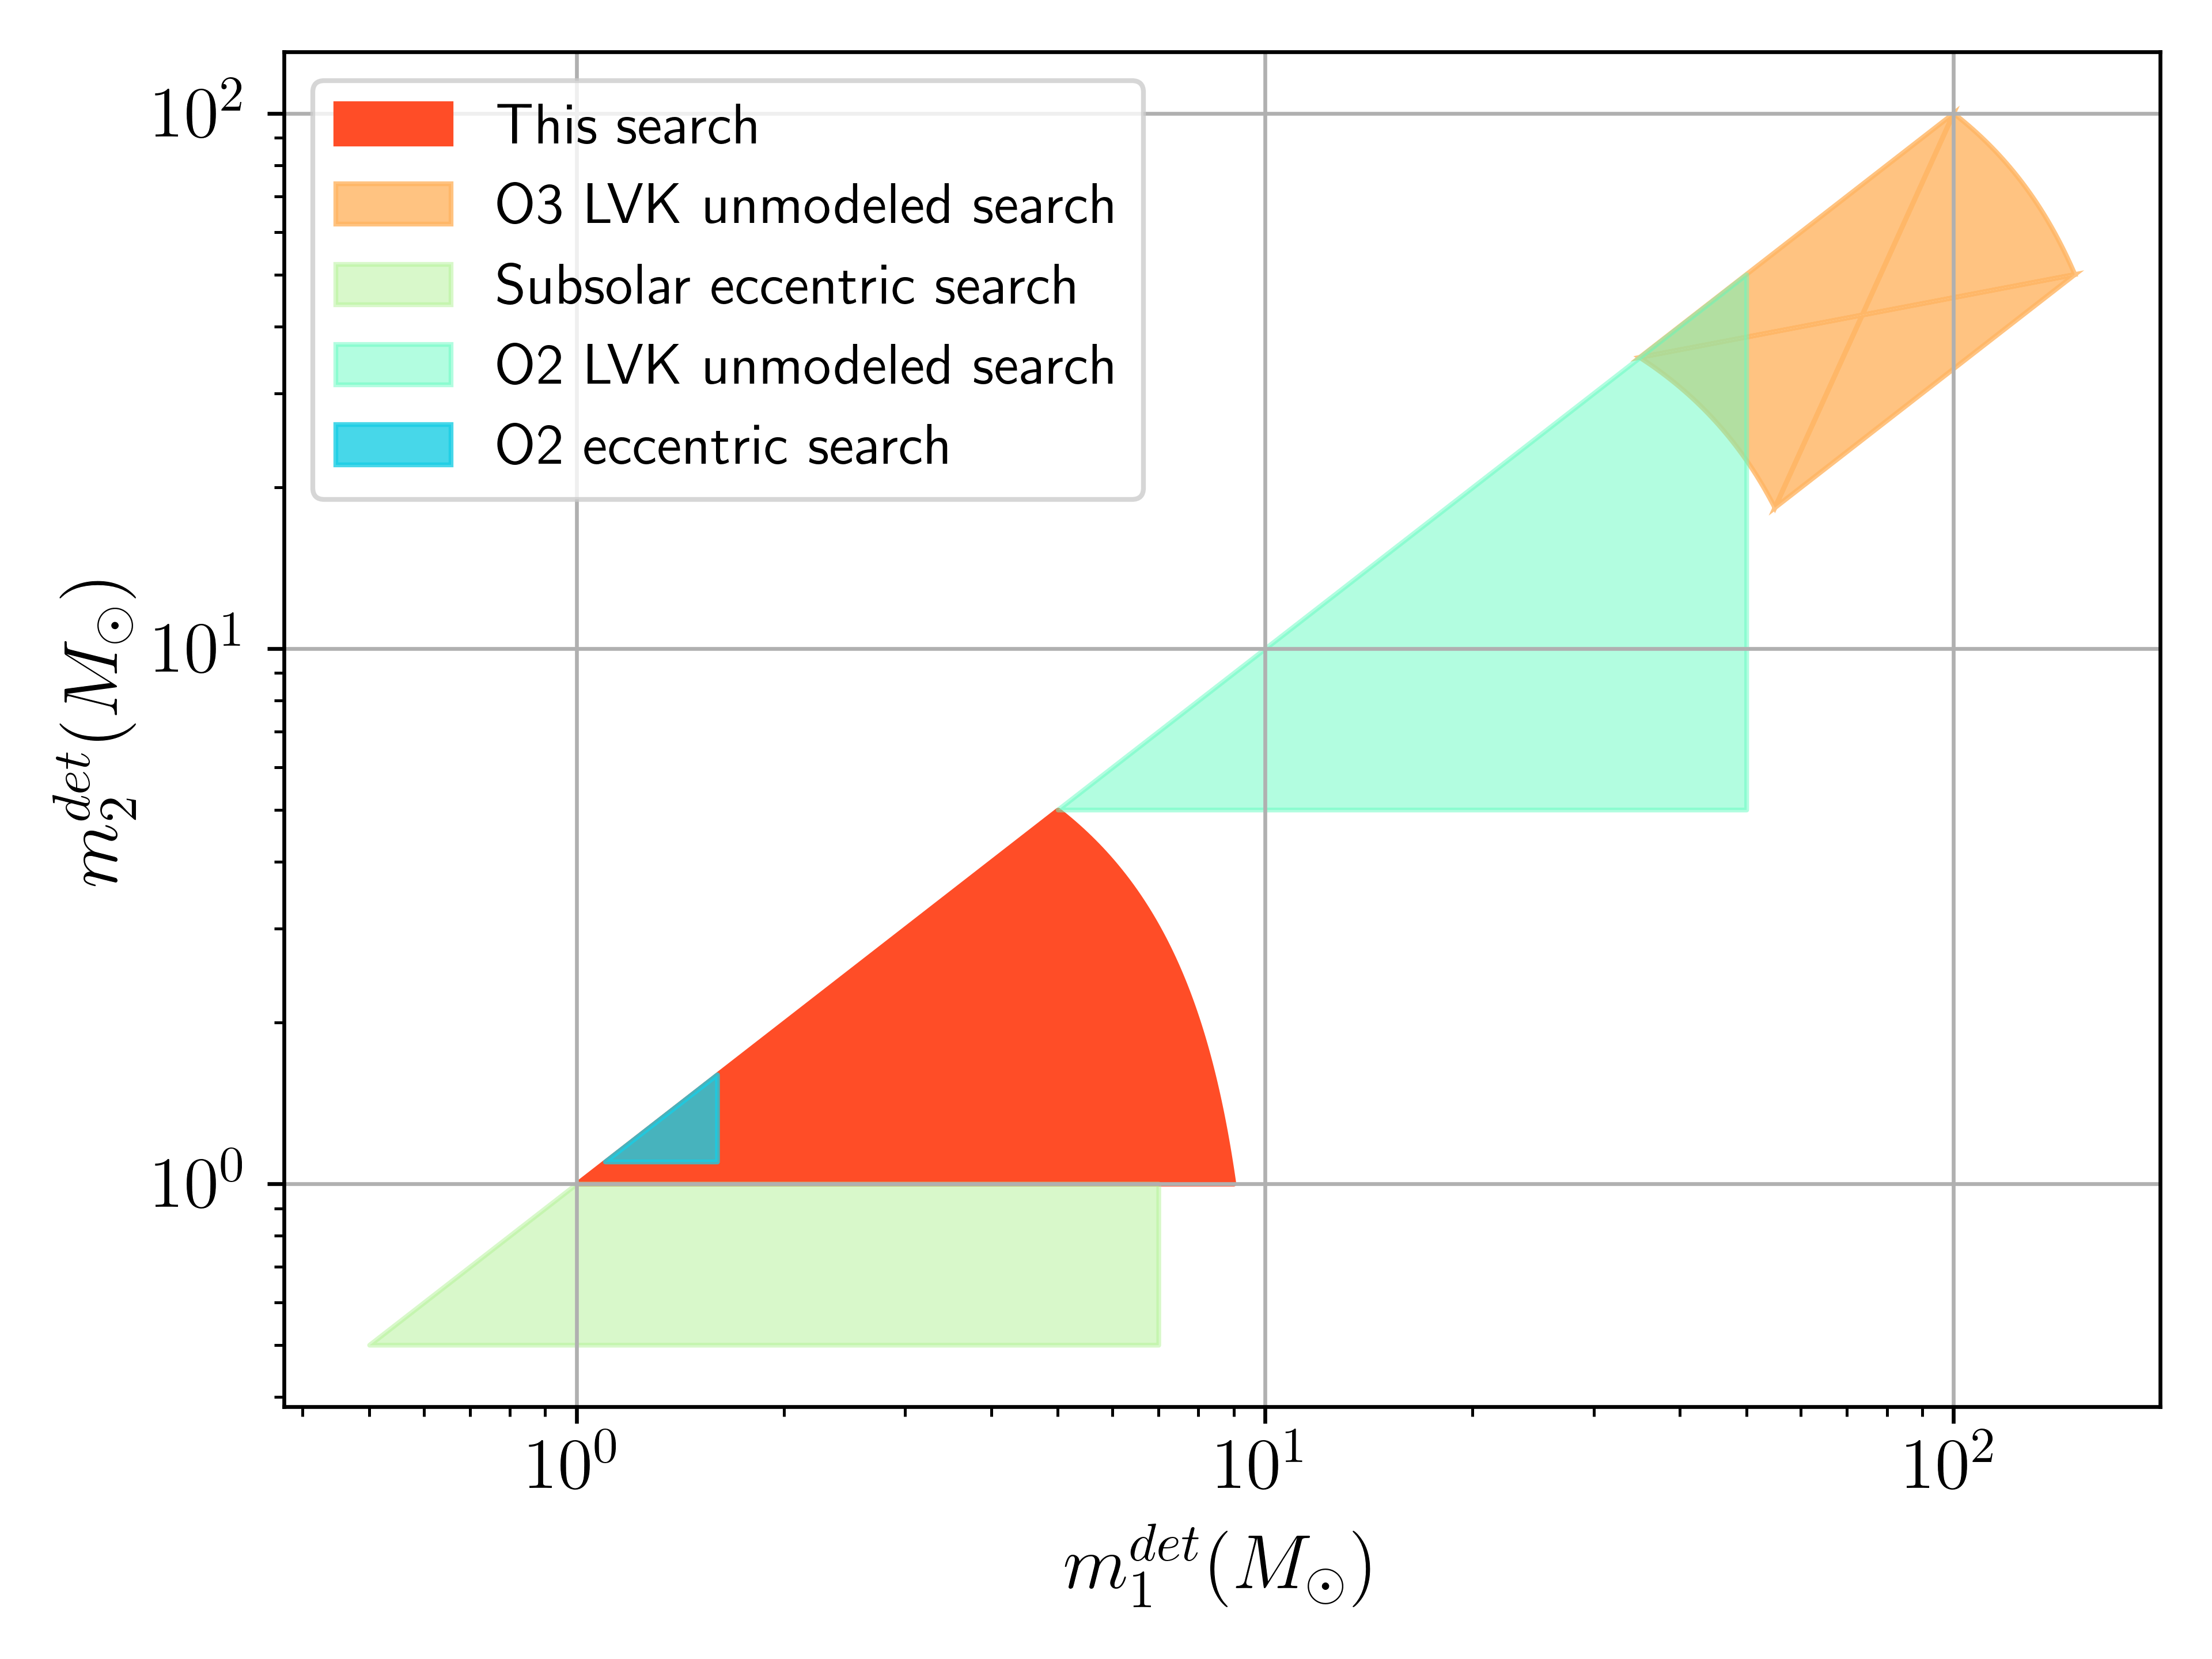
\includegraphics[width=\textwidth]{figures/ecc_search/Search_region.png}
    \caption{ Target regions of the various eccentric searches performed to date \cite{Nitz:2019spj,Nitz:2021vqh,LIGOScientific:2019dag,LIGOScientific:2023lpe} as a function of detector-frame masses ($m_1^{det}-m_2^{det}$). No prior searches have been explored for NSBH systems or BNS systems with spins. The prior search for BNS systems was restricted to a narrower region of masses and eccentricities ($e_{10} \leq 0.43$) and did not include spins \cite{Nitz:2019spj}. We search for spin-aligned neutron star binaries (BNS + NSBH) with eccentricities $e_{10} \leq 0.46$. The only searches for BBH sytems are unmodeled searches \cite{LIGOScientific:2019dag,LIGOScientific:2023lpe} and show the regions used to report their upper limits. The previous search for non spinning subsolar binaries restricted the eccentricities to $e_{10} \leq 0.3$ \cite{Nitz:2021vqh}.}
    \label{fig:search_region}
\end{figure}


\section{Search description and observational results}
To search for eccentric binaries, we use the PyCBC toolkit to perform a template-based matched filtering analysis to find modeled GW signals in the interferometric data \cite{Usman:2015kfa,Nitz:2017svb}. GW candidates are identified by finding peaks of the signal-to-noise (SNR) time-series, mitigating non-Gaussian noise artefacts, and checking the consistency of the data and astrophysical sources between each detector~\cite{Allen:2004gu, Nitz:2017lco,Davies:2020tsx}. Taking into account these factors and the empirically measure noise distribution, each candidate is assigned a ranking statistic value \cite{Nitz:2017svb, Davies:2020tsx, Was:2009vh}.

We search for neutron star binaries using a bank of modeled waveforms (templates) generated using a stochastic placement method \cite{Harry:2009ea,Babak:2008rb}. Our   
search region is described by five binary parameters: detector-frame component masses ($m_1^{det}, m_2^{det}$) ranging from [1.0, 9.0] $M_{\odot}$ with cutoff on total mass $M \leq 10 M_{\odot}$, $z-$ component of the individual spins ($\chi_{1z}, \chi_{2z} \in [-0.1, 0.1]$), eccentricity $e_{20}$ at 20 Hz $\in [0, 0.28]$, and an additional source orientation parameter $l$ related to the position of the periapsis. Our eccentric bank contains $\sim$ 6 million templates which is roughly two orders of magnitude larger than an equivalent bank for quasi-circular binaries. To model the GW signals, we use TaylorF2e inspiral only waveform model \cite{Moore:2016qxz} which accounts for eccentricity corrections to the aligned-spin quasi-circular TaylorF2 model \cite{Buonanno:2009zt}. Eccentricity causes phase and amplitude modulations of the GW signal, as shown in the Fig. (\ref{fig:ecc-WF}). Our search is reliably performed using only the inspiral part of the signal, since the merger falls outside the sensitive band of the current detectors. 

\begin{figure}
    \centering
    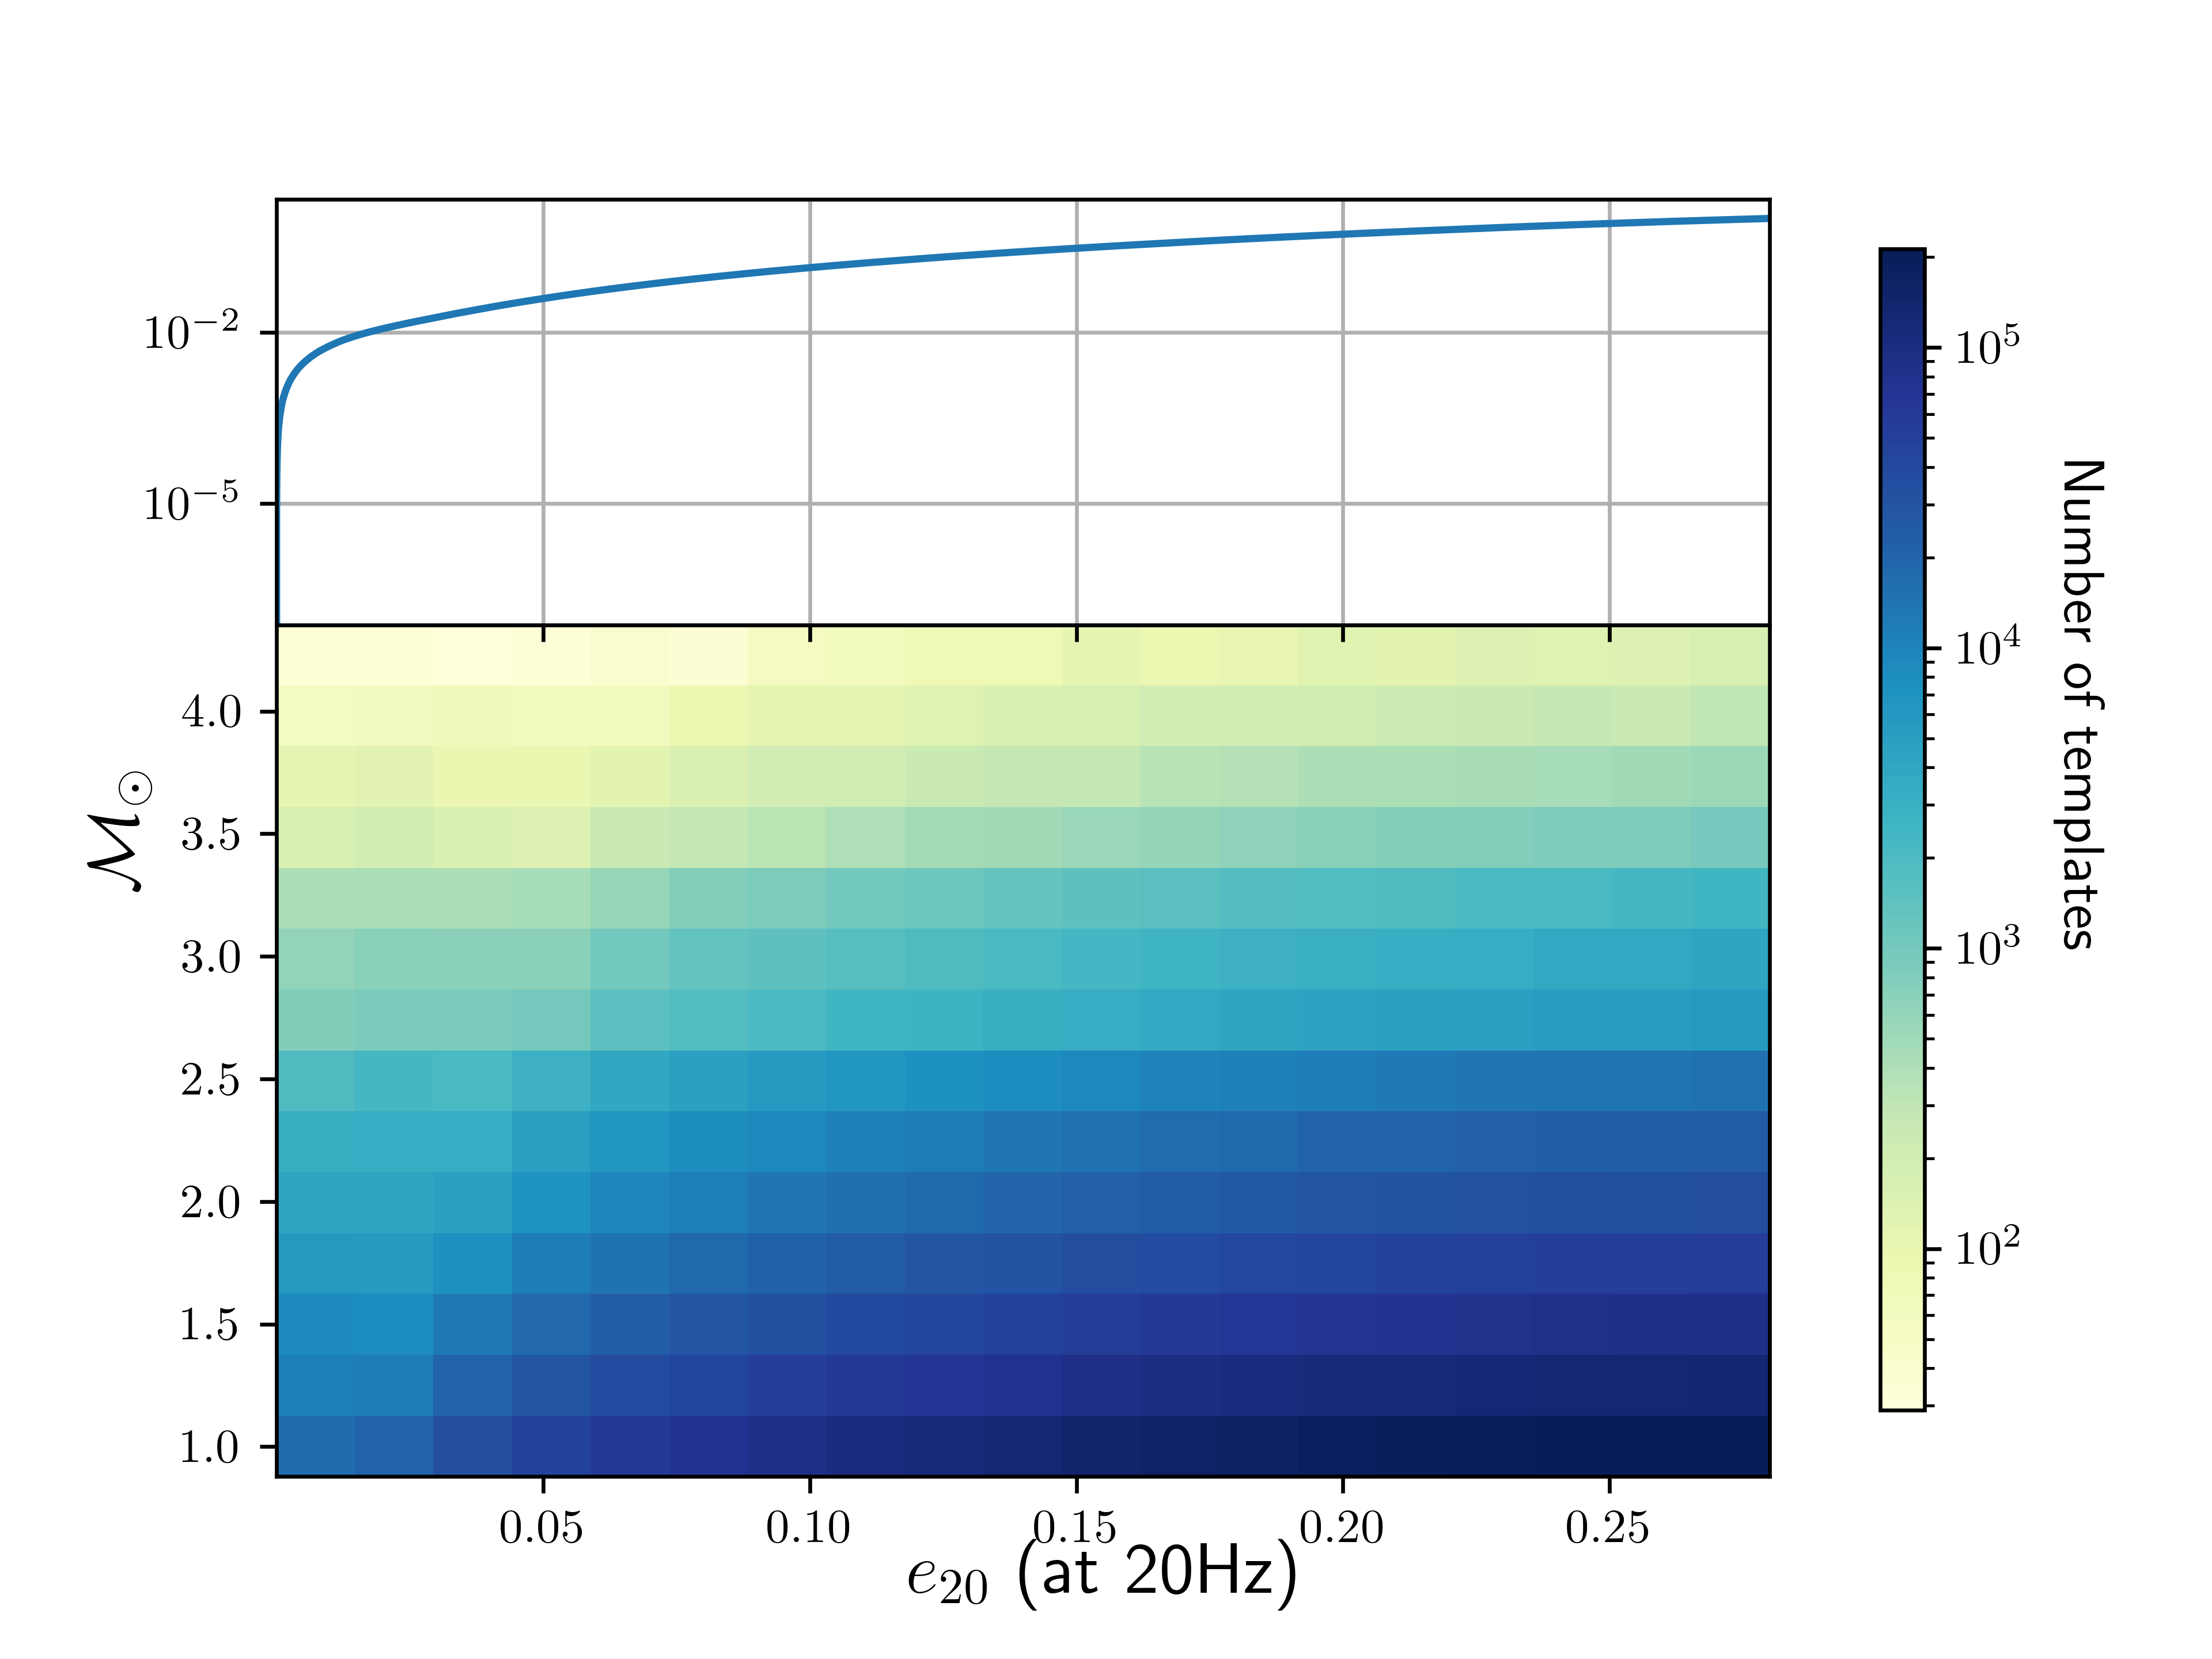
\includegraphics[width=\textwidth]{figures/ecc_search/bank_density.png}
    \caption{Our eccentric template bank as a function of the eccentricity at 20 Hz ($e_{10}$) and chirp mass. In the bottom panel we show the two dimensional binned histograms with the colorbar indicating the number of templates in each bin. The number of templates required to cover the parameter space increases with eccentricity -- our template bank contains $\sim 6$ million templates, an order of magnitude larger than an equivalent bank for circular binaries. In the top panel we show the cumulative distribution of templates as the function of eccentricity.}
    \label{fig:ecc-bank}
\end{figure}

\begin{figure}
    \centering
    \includegraphics[width=\textwidth]{figures/ecc_search/eccentric-wf.png}
    \caption{Effect of orbital eccentricity on the GW signal from $(10-10)M_{\odot}$ binary, two different scenarios are shown -- circular binary (pink) and eccentricity at 20 Hz ($e_{20} = 0.5$) (green). Eccentricity causes phase and amplitude modulations of the waveform. Eccentric binary radiates energy much quicker than a circular system, as evident by the shorter eccentric waveform.}
    \label{fig:ecc-WF}
\end{figure}


We search the O3 public Advanced LIGO and Virgo datasets using broadly the same search methods as \cite{Nitz:2021zwj}. O3 was divided into two parts -- O3a and O3b, comprising in total of $\sim 249$ days of coincident time when at least two observatories were in operation. Our search does not find any new significant GW candidates and recovered the previously reported multi-detector NSBH event GW200115 with high significance. The most significant candidate has a FAR of about 1 per year, consistent with the null hypothesis based on the observation duration. We show in the table \ref{tab:significant-events} the three most notable candidates, the list of top candidates, the template parameters associated with each candidate, and the configuration files necessary to reproduce the analysis are available in our data release~\cite{github}.  

\begin{table}[H]
    \centering
    \begin{tabular}{ccccccc}
        \hline
        \hline
         GPS time &  IFAR & $m_1$ & $m_2$ & $e_{10}$ & $\chi_{1z}$ & $\chi_{2z}$\\
         & (Yr)& $(M_{\odot})$ & $(M_{\odot})$ & & & \\
         \hline
         1247741648.397 & 1.02 & 1.56 & 1.02 & 0.36 & 0.04 & -0.07 \\
         1257948134.021 & 0.82 & 1.19 & 1.13 & 0.24 & -0.01 & -0.03 \\
         1265599361.194 & 0.43 & 2.95 & 1.03 & 0.22 & 0.05 & -0.08 \\
        \hline
    \end{tabular}
    \caption{Table of top three significant events from our search, sorted by the inverse false alarm rates (IFARs). The global positioning system (GPS) time of each candidate, the component mass $m_{1/2}$ (detector frame), eccentricity at $e_{10}$, and component spins $s_{1z/2z}$ of the template chosen by the search are shown.}
    \label{tab:significant-events}
\end{table}

We demonstrate the sensitivity of our search by the ability to recover a population of simulated sources as a function of luminosity distance $d_L$ for fixed chirp mass and orbital eccentricity $e_{10}$ averaged over sky locations and orientations. We generate the signals using the TaylorF2e approximant. Fig. \ref{fig:sensitive-dist} shows the average sensitive distance as a function of $e_{10}$ for four different values of $\mathcal{M}_c$. It is evident from the plot that sensitive distance scales linearly with the chirp mass and has a weak dependence on the eccentricity. As a comparison the sensitive distance for a fiducial $\mathcal{M}_c = 1.22 (1.4-1.4 M_{\odot})$ is improved from roughly 90 Mpc to 125 Mpc from O1/O2 to O3 run due to improvements in the current detectors. We point out the drop in sensitivity towards higher eccentricity because this region is outside of our search parameter space. 

\begin{figure}[h]
    \centering
    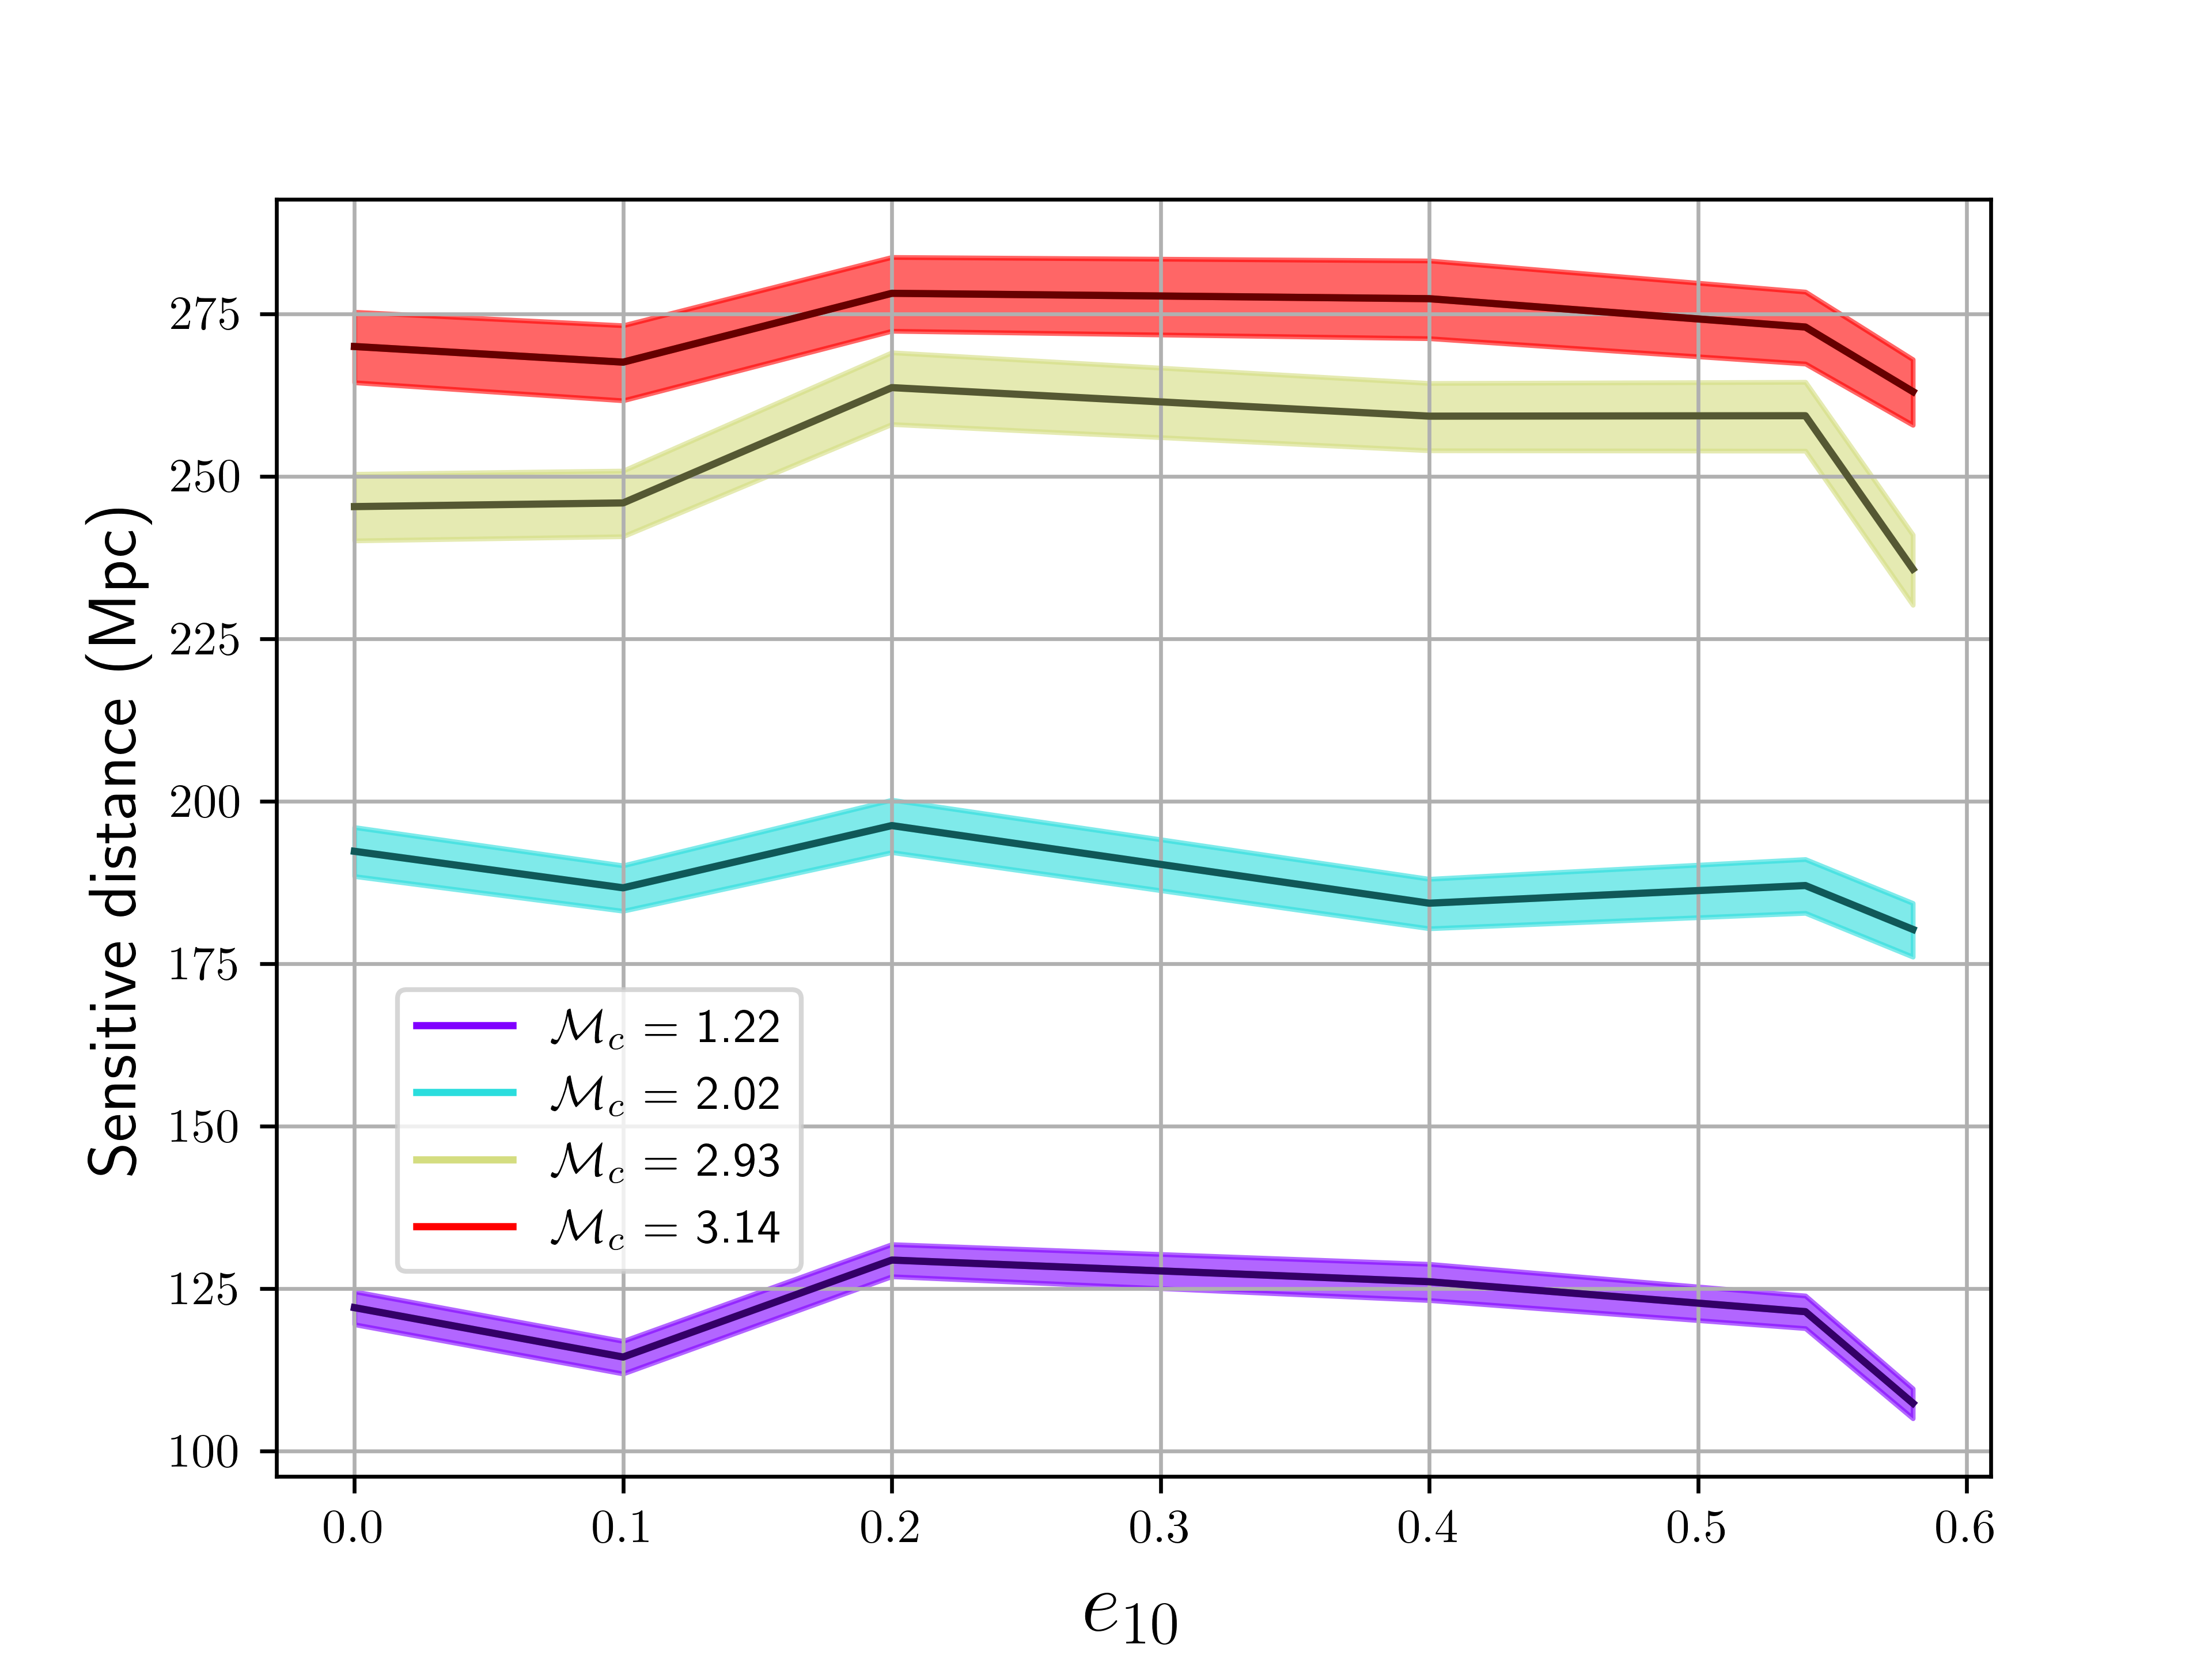
\includegraphics[width=\linewidth]{figures/ecc_search/SENS_DIST_ecc.png}
    \caption{Sensitive distance as a function of $e_{10}$ for systems with four different fixed $\mathcal{M}_c$ averaged over sky and orientation (Recast the axis to 10 Hz). The sensitive distance of our search is $\sim 1.3 \times$ better than previous eccentric BNS search due to the improvements in detector from O2 to O3. We remark that the sensitive distance increases with the chirp mass and varies weakly with eccentricity.}
    \label{fig:sensitive-dist}    
\end{figure}

\section{Constraining population models}

For a given astrophysical model with a merger rate density $\mathcal{R}(\theta, z)$, the expected number of detections within an observation period $T_{obs}$ is 
\begin{align}
    N_{detected} & = T_{obs} \int \int \mathcal{R}(\theta,z) f(\theta,z) \dfrac{dV_c}{dz}\dfrac{1}{1+z} d\theta dz ,
    \label{Eq:expected-detections}
\end{align}
where $p(\theta)$ is the distribution function of the binary parameters ($\theta$) predicted by an astrophysical model, $dV_c/dz$ is the differential co-moving volume and $f(z,\theta)$ is the probability of detecting a merger with $\theta$ parameters at a redshift $z$. We can constrain the local merger rate using the lack of observations: if we assume a Poisson distribution of observed mergers, then the 90\% confidence limit $R_{90}^{local}$ corresponds to a local merger rate when the expected number of detections is $\sim 2.3$ \cite{Biswas:2007ni}.


Upper limits are obtained by estimating the expected number of detections $N_{detected}$ (Eq. \ref{Eq:expected-detections}) via a Monte Carlo (MC) integration scheme for a synthetic population of mergers with binary parameter distributions predicted by the respective models \cite{Tiwari:2017ndi}. For a search, the detection probabilities can be estimated by using the search to detect simulated sources injected into the data. In our simulations, we assume the merger rate density follows the star formation rate \cite{Madau:2016jbv} convolved with the inverse time-delay distribution, same as the method used in \cite{Zhu:2020ffa, Wu:2022pyg}. The injection results from our search and the codes to estimate the observational limits are available as a part of our data release \cite{github}.  


\begin{sidewaysfigure}
    \centering
    \includegraphics[width=\textwidth]{figures/ecc_search/expected_ranges.png}
    \caption{ Predicted and observed constraints on the local merger rate for various populations of BNS and NSBH sources \cite{Belczynski:2017mqx, Sedda:2020wzl,Trani:2021tan,Fragione:2018yrb}. Assuming the observed neutron star binaries are part of the channels we considered, our measured rate (horizontal orange bars) is consistent with the observed rates in existing GW catalogs \cite{Nitz:2021zwj,LIGOScientific:2021djp,Olsen:2022pin}. The observational constraints assuming a null detection from our search for 249 days of observation is shown as blue (hatched) region. Predicted constraints for an idealized search are shown for O3 (blue), three $\text{A}^{\#}$ (green) and CE (40km) + CE (20km) (pink) for an year of observation. In an idealized search signals from high mass mergers can all be detected if they exceed a network SNR of 10: achieving this, our search constraints would be up to $5\times$ tighter reaching the idealized O3 limits (solid blue line). Next generation detectors will detect tens to hundreds of binaries, but not all would have sufficiently high eccentricities to be distinguished from non-eccentric binaries. When focusing on systems where $e_{10}\geq0.01$, the upper limits deteriorate inversely to the fraction of sources predicted by each model, affecting up to 80\% of NSBH systems from hierarchical triples or nuclear clusters. A fixed threshold does not capture the varied ability of different observatory networks to measure eccentricity. We further define a system with a measurable nonzero eccentricity if a non-eccentric model can be ruled out at the 90\% credible level. Using our predictions we can estimate the time required for an eccentric merger observation; the hierarchical triples model predicts a maximum merger rate of 0.34 $\text{Gpc}^{-3}\text{Yr}^{-1}$ and the $\text{A}^{\#}$ limit for systems with measurable eccentricity is 0.74 $\text{Gpc}^{-3}\text{Yr}^{-1}$, this gives an expected 2.2 years of observations with $\text{A}^{\#}$ for an eccentric NSBH merger observation. Three $\text{A}^{\#}$ will require 2 -- 100 years of observation to detect an eccentric NSBH merger for the range of models. CE will be able to detect mergers from every model and able to determine the eccentricity of tens to hundreds of binaries. This is even the case for isolated BNS mergers.
    } 
    \label{fig:time-requirement}    
\end{sidewaysfigure}

%%%%% Astrophysical constraints
\section{Astrophysical implications} 

We investigate how our observational results and the capability of future detectors can constraint four different astrophysical models: three dynamical pathways for NSBH systems within nuclear clusters \cite{Fragione:2018yrb}, globular clusters \cite{Sedda:2020wzl}, and hierarchical triples \cite{Trani:2021tan}, and a BNS formation model in the field \cite{Belczynski:2017mqx} to contrast the two major types of channels. The predicted merger rates of these models are shown in Fig. \ref{fig:time-requirement}. We constrain the local merger rate to be less than 150 $\text{Gpc}^{-3}\text{Yr}^{-1}$ (isolated BNS), 50 $\text{Gpc}^{-3}\text{Yr}^{-1}$ (NSBH in globular clusters), 100 $\text{Gpc}^{-3}\text{Yr}^{-1}$ (NSBH in hierarchical triples) and 70 $\text{Gpc}^{-3}\text{Yr}^{-1}$ (NSBH in nuclear clusters) under the assumption of non-detection from these channels. We also measure the rate of neutron star binaries from these models, assuming all prior observations are associated with each channel; these are consistent due to the lack of observations to date. Clearly, current GW observatories cannot constrain the dynamical formation models we have considered. 
%If we were to detect a highly eccentric merger it would necessitate a channel that can produce high eccentricities. 

Improved second generation and upcoming third generation observatories are expected to be a factor of a few and  more than an order of magnitude more sensitive than the current ones, respectively \cite{Asharp_sensitivity, CE_sensitivity}. Third generation detectors will be sensitive to the majority of neutron star binaries in the Universe. So the question arises: \textit{ To what extent can future observatories determine the formation history of neutron star binaries?} We predict how well upcoming second and third generation observatories will be able to constrain these models using an idealized search. We investigate constraints on the local merger rate for two networks (shown in Fig. \ref{fig:time-requirement}) -- one consisting of three $\text{A}^{\#}$ observatories and another composed of CE (40km) + CE (20km) using their expected noise curves \cite{Asharp_sensitivity, CE_sensitivity}. Furthermore, we have constraints for networks involving A+ and/or Einstein Telescope (ET) which are not presented here but are available in our data release \cite{github}. In agreement with \cite{Baibhav:2019gxm}, we find that CE will be able to detect majority of sources from each model. While current detectors may require up to $\mathcal{O}(10^3)$ years of observation to observe mergers from the considered dynamical formation models, three $\text{A}^{\#}$ observatories would begin detecting events from the most optimistic of these channels in roughly two years and CE (40km) + CE (20km) with a few days of observation.  
 
%Even when we are able to potentially observe binaries from each formation channel, only a fraction of binaries have sufficiently high eccentricities to distinguish them from non eccentric binaries: observations from future observatories may not be convincingly attributed to dynamical channels unless they have high eccentricity. 
Even though we can observe binaries from various formation channels, only those with high eccentricities can be clearly differentiated from non-eccentric binaries. Future observatory observations might struggle to confidently attribute binaries to dynamical channels unless they exhibit high eccentricity. To elucidate this, we show the population constraints for a fixed eccentricity threshold of $e_{10} \geq 0.01$ in Fig.~\ref{fig:time-requirement}. The limits for a fixed threshold scales inversely to the predicted fraction of systems satisfying this threshold: limits for mergers with $e_{10} \geq 0.01$ for NSBH in hierarchical triples or nuclear cluster models are worse only by a few factor due to large fraction of such sources predicted (see Fig. \ref{fig:eccentricity-dist}). 

The ability to measure eccentricity depends on the properties of a binary and the  \cite{Lower:2018seu} capabilities of a detector network, which a fixed threshold cannot capture -- we assess the potential of future observatories to measure eccentricity for each binary in our simulated population models. We determine the ability of a particular type of source to have non zero eccentricity using a simplified Bayesian analysis employing a Markov Chain Monte Carlo (MCMC) sampling scheme. We deem a source to have measurable eccentricity if at the 90\% credible level we can rule out the quasi-circular binary hypothesis. We find the threshold $e_{10} \geq 0.01$ falls short for measuring eccentric neutron star binaries with three $\text{A}^{\#}$ or for eccentric NSBH binaries with the CE network. In constrast, the CE network is more proficient in measuring eccentricities of BNS systems: the same threshold is overly optimistic for BNS.  Crucially, we find that third-generation observatories are poised to detect eccentric BNS systems even in isolated binary channels.

%Fig. \ref{fig:time-requirement} suggests that upcoming detector networks will detect many events from the given formation models, and a fraction of them will be eccentric observations which will enable a detailed study of their predicted eccentricity distributions.
Fig. \ref{fig:time-requirement} suggests that the CE detector network will observe hundreds of highly eccentric NSBH sources from nuclear clusters or hierarchical triples; their non-detection would require the channel to have lower merger rates, prompting tighter constraints on the model parameters. For example, in nuclear clusters, the distribution of stars around supermassive black holes (typically depicted by a power law $n(r) \propto r^{-\alpha}$) influences the eccentricity profile of NSBH systems \cite{Fragione:2018yrb}. An increase in $\alpha$ corresponds to more eccentric systems, so a non detection of eccentric sources would constrain the distribution of stars. CE will also measure eccentricities of isolated BNS mergers; with a model of natal orbital separations, one could estimate the distribution of natal eccentricities. Natal eccentricities are highly sensitive to the supernovae kick velocity \cite{Hobbs:2005yx, Richards:2022fnq}, and their estimation would allow constraints on the kick velocity.

\section{Conclusions}
We have performed a search for eccentric NSBH systems and the most sensitive search for eccentric BNS systems in the data from the third observing run (O3a + O3b) of Advanced LIGO and Advanced Virgo detectors. Our search did not find any new statistically significant merger candidates and as a result we put state-of-art upper limits on the local merger rates for an isolated BNS model and three distinct dynamical NSBH models:  150 $\text{Gpc}^{-3}\text{Yr}^{-1}$ (isolated BNS), 50 $\text{Gpc}^{-3}\text{Yr}^{-1}$ (NSBH in globular clusters), 100 $\text{Gpc}^{-3}\text{Yr}^{-1}$ (NSBH in hierarchical triples) and 70 $\text{Gpc}^{-3}\text{Yr}^{-1}$ (NSBH in nuclear clusters) assuming the prior neutron star binary observations do not belong to these models. While current observations are unable to constrain these models, the observation of a single highly eccentric source would have implications on the possible formation channels and suggest the presence of a dynamical formation mechanism.
%%Our current search is limited by the finite boundaries of our template bank and the lack of accurate high mass highly eccentric waveforms ~\cite{Nagar:2021gss,Ramos-Buades:2021adz}. 
An idealized search might be able to further tighten observational constraints on the total merger rate by $10 \%$ when all eccentricities and up to $\sim 5\times$ when all masses are modeled accurately. This motivates the development of models suitable at very high ($e_{10} \sim 0.8$) eccentricities, large mass ratio, and incorporating full models of their merger and ringdown. 

We make concrete predictions on how well upcoming detectors will be able to constrain formation models through observations of eccentric binary systems. A network of three $\text{A}^{\#}$ observatories and the combined capabilities of CE (40km) + CE (20km) will likely detect sources from these models. Our key results show that the CE detector network will identify eccentric NSBH sources within days of observation, while a network of $\text{A}^{\#}$ detectors might need anywhere between 2 to 100 years depending on the formation model considered.



\chapter{Sensitivity of spin-aligned searches for neutron star-black hole systems}

Current search methods are restricted to systems with quasi-circular orbits and only the dominant mode of the gravitational wave signals. These assumptions degrade the sensitivity for precessing NSBH mergers whose detections provides insights into their formation history. In this chapter, we explore our study of the sensitivity of current search methods for fully precessing NSBH mergers with higher-order modes of GW emission. We also explore how much current search assumptions affect the future observatories. Finally, we estimate the loss in sensitivity for an idealized precessing search.  The aim of this work is to identify the regions of parameter space strongly biased by the current searches and to motivate a target precessing search in those regions with current and future observatories.

\section{Introduction}
In the previous chapter, we discussed eccentricity as a signature of a binary's formation channel. Another signature is the spins of the components in a merger.  In scenarios where the binary components evolve together from their main sequence phase (like in the case of binary neutron stars or some black hole binaries), the spins are expected to be relatively well-aligned with the orbital angular momentum. This alignment can be due to the tidal interactions and mass transfer processes in the binary’s evolutionary history, which tend to align the spin axes of the components with the orbit. Conversely, in dense stellar environments like globular clusters or galactic nuclei, binaries can be formed through dynamical interactions. In such scenarios, the spins of the components are more likely to be misaligned with the orbital angular momentum which causes spin-induced precession of the binary orbit. This misalignment occurs because the binary components have independent evolutionary histories and are brought together by chance encounters rather than having evolved together. 

The latest catalogs of compact-object mergers reveal that a small number of these mergers display precession or higher-order modes. Notably, the BBH merger GW200129 has shown compelling signs of precession. Similarly, significant indications of higher-order mode emissions were observed in the events GW190814 and GW190412. Additionally, the ring-down analysis of GW190521 points to the presence of a less dominant mode.

The existing observations of NSBH and BBH mergers poses a challenge to different formation pathways and population synthesis models. Significant uncertainties in these models stem from the incomplete understanding of the binary environments such as distribution of stellar metallicity and physical process such as the dynamics of natal kicks. Identifying precessing NSBH mergers could play a crucial role in refining these models. Search strategies usually operate under the assumption that the spins of compact objects align with their orbital angular momentum, the orbits of these binaries are nearly circular, and only the primary mode $(l, m) = (2, 2)$ of gravitational wave emission is detectable. However, given that NSBH sources often have significant mass differences, it's anticipated that they could exhibit important higher-order modes. Moreover, if their black holes are rapidly spinning, noticeable precession could occur. Ignoring these factors in search methodologies might lead to pronounced biases in observations.  

Measuring spin precession presents significant challenges, particularly due to the detection of most sources at minimal inclination angles []. Furthermore, various studies indicate that deducing the spin precession parameter is complex, often influenced heavily by prior assumptions. Additionally, the substantial systematic differences in waveforms could lead to biased results in estimating the binary parameters. Measuring the higher-order modes of the signal alleviates some of the problems -- sub-dominant modes can carry information on spin-precession and including them in analysis helps break the mass-spin degenaracies [].

Past research has explored the efficacy of searches that focus solely on the dominant-mode of precessing events, as well as the biases that arise from overlooking precession and higher-order modes in binary black hole searches. These specialized searches demand a significantly higher number of templates more than $\sim 10\times$ compared to standard analyses. Due to the increase in the number of templates, such analyses produce a higher rate of false alarms at a fixed signal-to-noise (SNR) threshold. Thus, improvement in searches is driven by two competing effects -- higher SNR from precessing waveforms and larger trials factor. [] have found that searches for binaries with comparable component masses or near face-on systems do not benefit from incorporating misaligned spins or higher modes. However, up to $\sim 25\%$ of NSBH systems might be missed by aligned-spin searches. 

Modeling fast and accurate inspiral-merger-ringdown waveforms for fully precessing signals with relevant sub-dominant modes is an active field. There has been significant improvements to these models since the above mentioned studies were performed. In this work, we use the state-of-art precessing IMR waveforms to compare the sensitivity of spin aligned searches in Advanced LIGO, $A^{\#}$, LIGO Voyager and Cosmic Explorer. We determine the fraction of sources that would be detected by a dominant-mode, aligned-spin search compared to the ideal search that fully accounts for precession and higher-order mode.   


Owing to the inherent challenges associated with each of these methodologies, no search that includes waveforms factoring in precessional effects has been conducted using the data from Advanced LIGO, Advanced Virgo, or KAGRA. Efforts are underway for developing a fully precessing search. A completely different methodology of searching precessing systems using     

\section{Modeling precessing CBC signals with HMs}

Numerous models are available to describe the complete inspiral, merger, and ringdown parts in the gravitational wave signals from compact-binaries. These models are capable of incorporating spin-precession effects and higher-order modes of the signal. They are generally divided into three main categories: phenomenological models, effective one-body numerical relativity (EOBNR) models, and surrogate models. Current searches employ waveform models from both the phenomenological and effective-one body families. Given that our study is focused on the efficacy of model-based searches, we will provide a concise overview of the signal model. 

We revist the quasi-circular CBC signal model that can be characterized by 15 parameters. These parameters are broadly divided as 1. \uline{\textit{Intrinsic parameters}} $\kappa$: the component masses $(m_1, m_2)$ and component spin vectors $(\Vec{\chi_1}, \Vec{\chi_2})$, and the 2. \underline{\textit{Extrinsic parameters}}: the sky-location angles ($\alpha, \delta$) in the frame of the observer, luminosity distance $d_L$, the inclination angle $i$ between the orbital angular momentum \textbf{L} and the line of sight to the observer, polarization angle $\psi$, the time of coalescence $t_c$ and the orbital phase $\phi_c$ of the binary.

The gravitational wave $h(t)$ as seen by a detector is a linear combination of the two gravitational-wave polarization
\begin{align} 
    \begin{aligned}
    h(t) = F_{+}(\alpha, \delta, \psi) & h_{+}(\kappa, i, d_L, \varphi_c; t) \\ & + F_{\times}(\alpha, \delta, \psi)h_{\times}(\kappa, i, d_L, \varphi_c; t),
    \end{aligned}
    \label{Eq:Detector_response}
\end{align}

where the coefficients $F_{+}$ and $F_{\times}$ are the time-independent antenna pattern functions of the detector \cite{Finn:1992xs, Jaranowski:1998qm}. The two polarization are defined in the radiation frame and together they make up the complex strain $H = h_{+} + i h_{\times}$. This complex strain can be further decomposed using the spin-2 weighted spherical harmonics $Y^{-2}_{lm}$ \cite{Spin-weighted-harmonics}
\begin{align}
        \label{Eq:spherical_harmonics}
    H \equiv h_+ + ih_{\times} = \sum_{l\geq2}\sum_{m=-l}^{m=l} Y^{-2}_{l,m}(i, \varphi_c) h_{l,m}(\kappa, d_L ;t-t_c),
\end{align}
where the $h_{l,m}$ are the various \textit{modes} of the GW signal which are function of $\kappa, d_L$ and $t_c$. These various modes  (explicit expression can be found in \cite{Mills:2020thr})) have different contributions to the observed signal via the respective $Y^{-2}_{l,m}(i, \varphi_c)$. The dominant mode $(l,m)$ = (2,2) is the strongest at face-on ($i=0$) or face-off ($i = \pi/2$) configurations and grows fainter with increasing $i$ reaching minimum at $i = \pi/2$. However, significantly inclined binaries can have stronger higher modes. In general for a given mode ($l, m$), we can write  
\begin{align}
    h_{l,m}(\kappa, d_L; t) = A_{l,m}(\kappa, d_L; t)e^{-i\Phi_{l,m}(\kappa;t)},
    \label{Eq:single_mode}
\end{align} 
where $A_{l,m}, \Phi_{l,m}$ are respectively the real amplitude and phase for a given mode. The phase $\Phi_{l, m}$ for each mode is related to the orbital phase as $\Phi_{l,m}(t) = m\phi_{orb}(t)$ up to a good approximation ~\cite{Apostolatos:1994mx}, which depends strongly on the component spins.

The individual modes $h_{l,m}$ are functions of the spin parameters.
We denote the spin angular momenta $\textbf{S}_1 = \vec{\chi}_1 m_1^2$ and $\textbf{S}_2= \vec{\chi}_2 m_2^2$.  In the case of aligned-spin systems, the direction of the orbital angular momentum remains fixed and thus, $\textbf{S}_1 \textbf{S}_2$, and $\textbf{L}$ are parallel. In the case of systems with generically oriented spin vectors, the spins of the compact objects couple with the orbital angular momentum which may cause spin-precession. For such systems, the orbital angular momentum $\textbf{L}$ precesses around the nearly fixed total angular momentum $\textbf{J} = \textbf{S}_1 + \textbf{S}_2 + \textbf{L}$; the inclination angle varies over time. The various spin and orientation angles are shown in the Fig. \ref{fig:precessing_angles}. Note, even though $\textbf{J}$ is considered to be fixed to a good approximation \cite{Apostolatos:1994mx}, there can be rare instances where $\textbf{J}$ can change significantly \cite{Apostolatos:1994mx}. 

\begin{figure}[]
    \centering
    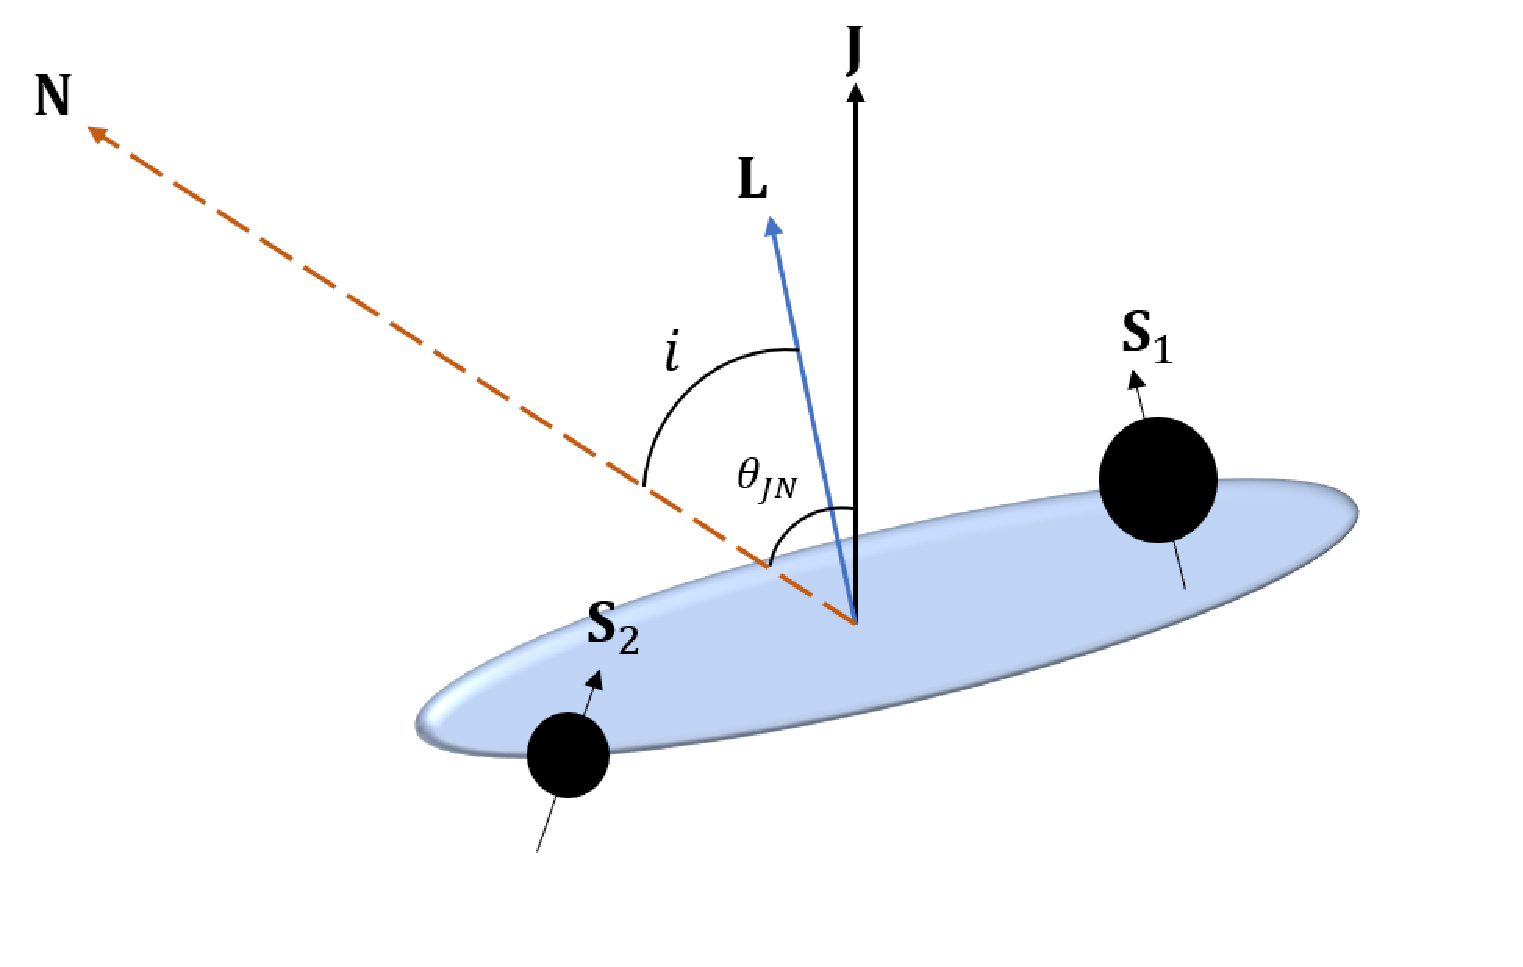
\includegraphics[width=10cm]{figures/HM_and_precession/Precessing_angles.pdf}
    \caption{The angular momentum vectors for a precessing binary. The inclination angle $i$ is defined as the angle between the orbital angular momentum $\textbf{L}$ and the line of sight to the observer $\textbf{N}$. The angle between $\textbf{J}$ and $\textbf{N}$ is denoted as $\theta_{JN}$. Due to spin-orbit coupling, $\textbf{L}$ and $\textbf{S}$ will precess around the approximately fixed $\textbf{J}$.} 
    \label{fig:precessing_angles}
\end{figure}

Precession dynamics cause phase and amplitude modulations to the observed signal. Since precession is caused by the non-alignment of the spins with the orbital angular momentum, to measure the strength of precession, it is common to group the in-plane and parallel spin components. The spin effects are commonly characterized in terms of the two effective parameters \cite{Ajith:2009bn, Schmidt:2014iyl}

\begin{align}
    \chi_{\text{eff}} = \dfrac{1}{M}\Bigg(\dfrac{\textbf{S}_1}{m_1}+\dfrac{\textbf{S}_2}{m_2}\Bigg)\cdot\hat{\textbf{L}}, \label{eq:chi_eff}\\
    \chi_{p} = \dfrac{1}{A_1m_1^2}\max\Big(A_1 S_1^{\perp},A_2 S_2^{\perp}\Big), \label{eq:chi_P}
\end{align} 

where, $A_1=2+3q/2$ and $A_2 = 2 + 3/(2q)$, $q$ is the mass-ratio $m_1/m_2$, and $S_i^{\perp}$ is the projection of the spins orthogonal to $\textbf{L}$. The $\chi_{\text{eff}}$ parameter gives us a measure of the spin components parallel to $\textbf{L}$. The four in-plane spin components are averaged over a precessing cycle to obtain an effective $\chi_p$ precession parameter.

\section{ Reference NSBH population } \label{sec:ref_pop}
Since the precession and higher order-mode effects grow with mass-ratio, we choose to study a population of NSBH source extending up to $q = 20$ with the broad priors shown in table~\ref{tab:priors}. We sample the component masses in terms of the detector frame masses $m_{1,2}^{det} = (1+z)m_{1,2}$, where $z$ is the redshift of a source. The redshifted masses are sampled uniformly between $5 M_{\odot} \leq m_1^{det} \leq 30 M_{\odot}$ and $1 M_{\odot} \leq m_2^{det} \leq 3 M_{\odot}$. Working in the detector frame eliminates the redshift dependence in the calculation of signal-to-noise ratio and related metrics (see e.g. sec \ref{sec:metrics}).


We choose the spin directions to be isotropically distributed and the spin magnitudes to be uniform. We assume neutron-stars are slowly spinning with spin-magnitude up to 0.05, and up to one for black-holes. We also assume the sources are isotropically distributed in the sky. The polarization angle, coalescence phase and the cosine of the inclination angle are also uniformly distributed. In total we simulate a population of 50,000 compact-binaries.

In this study, we employ one of the latest models from the phenomenological waveform family \approximant{IMRPhenomXPHM} \cite{Pratten:2020ceb} to generate signals for our fiducial population. This model accounts for generic spins and HMs and includes $(l, |m|) = (2, 2), (2, 1), (3, 3), (3, 2), (4, 4)$ modes. \approximant{IMRPhenomXPHM} has shown consistent results with other waveform models in the recent compact-merger catalogs \cite{LIGOScientific:2021djp, Nitz:2021uxj, Olsen:2022pin}, inference studies of various GW events \cite{Estelles:2021jnz, Krishnendu:2021cyi}, and studies inferring population properties \cite{Tiwari:2021yvr, Zhu:2021jbw}. Thus, the reliability and computational efficiency of \approximant{IMRPhenomXPHM} motivated us to employ this model.  

\begin{table}[]
    \centering
    \begin{tabular}{c|c}
        Parameter &  Distribution\\
        \hline
        \hline
        $ m_{1}^{det} $ & uniform $\in$ [5.0, 30.0]  $ M_{\odot}$ \\
        \hline
        $ m_{2}^{det} $ & uniform $\in$ [1.0, 3.0] $ M_{\odot} $\\
        \hline 
        $\abs{\chi_{1}}$ & uniform $\in$ [0, 1] \\
        \hline
        $\abs{\chi_{2}}$ & uniform $\in$ [0, 0.05] \\
        \hline
        Spin tilt angles & Isotropic\\
        \hline 
        Sky angles & Isotropic \\
        \hline
        $\varphi_c$ & uniform $\in$ [0, $2\pi$]\\
        \hline
        $\cos{i}$ & uniform $\in$ [-1, 1] \\
        \hline
        $\psi$ & uniform $\in$ [0, $2\pi$]
    \end{tabular}
    \caption{ Various source parameters (first column) used in the simulation for the reference NSBH population consisting of 50,000 compact-binaries. The second column shows the distribution used to sample the corresponding parameter.}
    \label{tab:priors}
\end{table}

\section{}

\chapter{A novel method to reduce computational costs of modeled searches : Hierarchical matched filtering using a reduced basis}

\chapter{Conclusions and future work}

In this thesis, we explored the prospects of detecting two significant astrophysical phenomena: binaries in eccentric orbits and those with precessing orbital planes. We have performed a search for spinning eccentric neutron star binaries. A core component of this thesis motivates the search of eccentric and precessing binaries in the future. We have made predictions for eccentric observations for networks of second and third generation observatories. Furthermore, the necessity of searching for precessing binaries is underscored by pinpointing areas in the parameter space where current methods exhibit low sensitivity to such systems. Recognizing the potential computational demands of these searches, we have introduced an innovative approach to reduce computational expenses in matched filtering.

%Observation of a clearly eccentric or precessing binary system are crucial for determining the formation history and constraining uncertainties in various astrophysical models. To date there has been only one event with strong evidence for orbital precession and none for orbital eccentricity. Current state-of-art search methods have primarily focused on non-precessing, quasi circular binaries. To tackle these issues, we have explored three different avenues. In Chapter 4, using simple extension of current search methods and inspiral only eccentric waveforms, allowed us to reliably search for eccentric neutron star binaries. No new significant candidate was found, but we put the most stringent constraints for four different binary formation scenarios and predicted the capabilities of future detectors to use eccentric observations in determining the formation channels of compact binaries.  In Chapter 5, we shifted our focus to the next signature -- orbital precession. Extension of current search pipelines for precessing system is an ongoing effort, thus, to motivate future searches we have identified regions of the NSBH parameter space that are worst affected due to simplifying search assumptions, and quantify loss in sensitivity in these regions. Finally, in Chapter 6, we have tackled a challenge common to both search scenarios which is the increased computational costs for searching exceptional events by, that restricts our capability to search for new sources in a wide parameter region. Searches with future detectors are also expected to increased computational costs which will become challenging. We demonstrated our new hierarchical matched filtering using reduced basis to drastically reduce the costs of matched filtering. Furthermore, we have shown implementing this scheme on GPU can have significant commercial benefits. 


The key takeaways from this thesis are as follows.  While current observatories require a serendipitous detection of an eccentric system, improved second generation and future third generation observatories will be able to observe binaries even from dynamical formation channels. A fraction of these binaries will have measurable eccentricities, and we predict, observation of a clearly eccentric signal would require at least two years of observation with a network of three $A^{\#}$ and at least ten days with a network of Cosmic Explorers. Current searches are losing up to 24$\%$ of sources with mass ratios $q > 6$ and up to $\sim 60\%$ of highly precessing sources $\chi_P > 0.5$. Conducting searches for novel binaries or utilizing future observatories presents significant computational challenges. Using hierarchical search methods shows a potential reduction in floating-point operations by up to $\sim 10\times$. Furthermore, using GPUs for these searches is up to 100 times more energy and cost-effective, highlighting the crucial role of GPUs in gravitational wave detection efforts.


Improvements to the second generation and the upcoming third generation observatories are expected to be operational in the early to mid 2030s. These new detectors are set to revolutionize the field by exponentially increasing the number of observed GW events from around  $\mathcal{O}(100)$ as seen with the second-generation observatories up to $\mathcal{O}(10^5)$. This expected surge in observations will necessitate considerable efforts in various areas ranging from theoretical models to data analysis techniques. This is when our search methods and waveform models should be on par to capture novel binary events, that will be able to answer some of the most awaited answers in astronomy, astrophysics and physics. 

Eccentricity and precession can exhibit similar characteristics \cite{Romero-Shaw:2022fbf}, leading to difficulties in distinguishing their respective influences on formation channels. The optimal strategy for developing waveform approximants that account for both non-zero eccentricity and precession involves creating a surrogate model based on a set of eccentric and precessing numerical relativity waveforms. However, this approach is likely several years away from being feasible. The challenge lies in the scarcity of numerical relativity waveforms that are both eccentric and precessing, coupled with the fact that generating these simulations requires considerable time and energy. In the interim, until dependable waveform models become available, our focus will remain on exploring new binary searches. We will propose three different future prospects of research based on the extension of works in this thesis below. 


Eccentric BBHs have been only searched using the less sensitive unmodeled searches. This is due to lack of fast IMR eccentric waveforms -- the merger is in the sensitive band of the current detectors and thus, a modeled eccentric search for BBHs also requires the merger and the ringdown part. Rapid development is underway to make faster, eccentric IMR waveform models that cover a wide parameter range \cite{Klein:2021jtd, Joshi:2022ocr}. With such models available, we aim to perform the first modeled eccentric BBH search using the publicly available data. The prospects of observing a clearly eccentric BBH may be slightly better due to higher detection rate for BBHs compared to neutron star. Constraints on dense star cluster will become significantly tighter with 10 eccentric BBH observations \cite{Zevin:2021rtf}.      

Efforts for developing search methods for precessing system is currently underway, involving decomposition of precessing waveforms \cite{McIsaac:2023ijd,Fairhurst:2019vut}. A search method using original precessing waveforms has to address several problems. First, is defining the parameters to be included in the template bank. Second, is to define the coincidence between any two detectors -- the condition of exact-match coincidence is no longer valid, because a precessing signal may be triggered with different template parameters in different detectors. We plan to develop a precessing search method by implementing a two-stage hierarchical scheme that will use a coarser template bank for the first-stage and then a follow-up with a rapid parameter estimation. We intend to use the component masses, the effective spin parameters, the inclination angle and an extra angle to be included in the template bank. Triggers only from the same bank will be followed up for the coincidence test. 

% 
Searches for sub-solar or low-mass binary systems provide a wealth of information on the equation of state of dense nuclear matter, dark matter or new physics \cite{Nitz:2022ltl,LIGOScientific:2022hai}. The detection of a subsolar-mass black hole would definitively confirm the existence of Primordial Black Holes (PBHs), which are candidate for dark matter \cite{Sasaki:2018dmp, Carr:2020gox}. Detecting a low-mass neutron star would provide valuable constraints on the equation of state of dense nuclear matter \cite{Silva:2016myw}. However, as previously mentioned, the search for these low-mass binaries demands substantial computational resources. Furthermore, incorporating tidal deformabilities to potentially enhance the sensitive volume by approximately $80\%$ \cite{Bandopadhyay:2022tbi}, would significantly escalate the search costs. This challenge further motivates the need for applying our hierarchical matched-filtering approach. We plan to integrate this method into the PyCBC search pipeline, enabling more cost-effective and energy-efficient execution of any modeled search.

%Search for sub-solar binaries can provide constraints on primordial black hole population, which are candidates. Sub-solar binaries can be attributed to primordial black hole population, which are candidate for dark matter \cite{}.   Sub-solar or low-mass compact objects may consist of primordial black holes (PBH)s \cite{}. PBHs are candidates for dark matter, and searching for low-mass binaries could provide further insights \cite{}.


%No pior searches for precessing system and no modeled searches for eccentric BBH systems have been performed to date. This means a large parameter space remains unexplored to look for these systems. As mentioned earlier, one of the issues in searching for these systems is the large amount of computational resources required, which can be tackled by our new matched filtering scheme. In future we plan to integrate our method into the standard PyCBC search pipeline and perform a hierarchical search for precessing systems targeting the regions of poor sensitivity identified in our study. Other limitation is the lack of fast and accurate eccentric IMR waveforms which prohibit us from searching for eccentric BBH models. However, currently a model is being developed which is expected to be accurate and fast enough for us to perform an eccentric BBH search soon.


   



%Challenges
%suffers from lack of fast, accurate eccentric waveforms and in case of precessing binaries,


%\printbibliography[heading=bibintoc]
\begin{sloppy}
\printbibliography
\end{sloppy}

\appendix

\chapter{Acknowledgments}
Thenks

%\chapter{Catalog of events from 4-OGC}

 \setlength{\LTcapwidth}{\textwidth}
\begin{longtable}{cccccccccc}
  \caption{Shown are the gravitational-wave observations from the full search on data from O1-O3 with $\mathcal{P}_{\textrm{astro}} > 0.5$ or IFAR $>$ 100 years sorted by observation time. We list the GPS time for each event alongside information on the observational status of the three observatories LIGO Hanford (H), LIGO Livingston (L), and Virgo (V). We also list the detectors for which our search triggered and the corresponding recovered SNRs ($\rho$). For some events, where multiple detectors are operational, the search does not trigger for all observatories. This is caused by requiring consistency of the triggers between detectors and triggers in individual detectors needing to exceed the SNR threshold. For multi-detector events we provide the IFAR at the associated ranking statistic for the event. The probability of astrophysical origin is estimated for all events detected by the focused BBH search and from the single-detector analyses. Events reported here for the first time are marked by bold font.}
\label{table:search}\\
 & Event & GPS Time & Observing & Triggered & $\mathcal{P}_\textrm{astro}$ & IFAR [yr] & $\rho_H$ &  $\rho_L$  & $\rho_V$  \\\hline
    \endfirsthead
  \caption*{(Continued) Shown are the gravitational-wave observations from the full search on data from O1-O3 with $\mathcal{P}_{\textrm{astro}} > 0.5$ or IFAR $>$ 100 years sorted by observation time. We list the GPS time for each event alongside information on the observational status of the three observatories LIGO Hanford (H), LIGO Livingston (L), and Virgo (V). We also list the detectors for which our search triggered and the corresponding recovered SNRs ($\rho$). For some events, where multiple detectors are operational, the search does not trigger for all observatories. This is caused by requiring consistency of the triggers between detectors and triggers in individual detectors needing to exceed the SNR threshold. For multi-detector events we provide the IFAR at the associated ranking statistic for the event. The probability of astrophysical origin is estimated for all events detected by the focused BBH search and from the single-detector analyses. Events reported here for the first time are marked by bold font.}
      \label{table:search}\\
 & Event & GPS Time & Observing & Triggered & $\mathcal{P}_\textrm{astro}$ & IFAR [yr] & $\rho_H$ &  $\rho_L$  & $\rho_V$  \\\hline
    \endhead 
    \hline
    \endfoot
 1 & GW150914\_095045 & 1126259462.43 & HL & HL & 1.00 & $>100$ & 19.9 & 13.0 & - \\
\rowcolor{gray!20} 2 & GW151012\_095443 & 1128678900.45 & HL & HL & 1.00 & $>100$ & 6.9 & 6.6 & - \\
\rowcolor{white} 3 & GW151226\_033853 & 1135136350.65 & HL & HL & 1.00 & $>100$ & 10.5 & 7.4 & - \\
\rowcolor{gray!20} 4 & GW170104\_101158 & 1167559936.60 & HL & HL & 1.00 & $>100$ & 8.9 & 9.6 & - \\
\rowcolor{white} 5 & GW170121\_212536 & 1169069154.58 & HL & HL & 1.00 & 16 & 5.2 & 8.9 & - \\
\rowcolor{gray!20} 6 & GW170202\_135657 & 1170079035.73 & HL & HL & 0.86 & 0.50 & 5.4 & 6.2 & - \\
\rowcolor{white} 7 & GW170304\_163753 & 1172680691.37 & HL & HL & 0.74 & 0.25 & 4.6 & 7.0 & - \\
\rowcolor{gray!20} 8 & GW170403\_230611 & 1175295989.23 & HL & HL & 0.72 & 0.25 & 5.2 & 5.5 & - \\
\rowcolor{white} 9 & GW170608\_020116 & 1180922494.49 & HL & HL & 1.00 & $>100$ & 12.4 & 9.0 & - \\
\rowcolor{gray!20} 10 & GW170727\_010430 & 1185152688.03 & HL & HL & 1.00 & 71 & 4.7 & 7.5 & - \\
\rowcolor{white} 11 & GW170729\_185629 & 1185389807.32 & HL & HL & 1.00 & 28 & 7.5 & 6.9 & - \\
\rowcolor{gray!20} 12 & GW170809\_082821 & 1186302519.75 & HLV & HL & 1.00 & $>100$ & 6.7 & 10.7 & - \\
\rowcolor{white} 13 & GW170814\_103043 & 1186741861.53 & HLV & HL & 1.00 & $>100$ & 9.2 & 13.7 & - \\
\rowcolor{gray!20} 14 & GW170817\_124104 & 1187008882.45 & HLV & HL & - & $>100$ & 18.3 & 25.5 & - \\
\rowcolor{white} 15 & GW170818\_022509 & 1187058327.08 & HLV & HL & 1.00 & 5.26 & 4.5 & 9.6 & - \\
\rowcolor{gray!20} 16 & GW170823\_131358 & 1187529256.52 & HL & HL & 1.00 & $>100$ & 6.6 & 9.1 & - \\
\rowcolor{white} 17 & GW190404\_142514 & 1238423132.99 & HL & HL & 0.50 & 0.02 & 5.1 & 5.9 & - \\
\rowcolor{gray!20} 18 & GW190408\_181802 & 1238782700.28 & HLV & HL & 1.00 & $>100$ & 9.2 & 10.3 & - \\
\rowcolor{white} 19 & GW190412\_053044 & 1239082262.17 & HLV & HL & 1.00 & $>100$ & 8.2 & 14.9 & - \\
\rowcolor{gray!20} 20 & GW190413\_052954 & 1239168612.50 & HLV & HL & 1.00 & 1.45 & 5.2 & 6.7 & - \\
\rowcolor{white} 21 & GW190413\_134308 & 1239198206.74 & HLV & HL & 1.00 & 6.39 & 5.4 & 7.8 & - \\
\rowcolor{gray!20} 22 & GW190421\_213856 & 1239917954.25 & HL & HL & 1.00 & $>100$ & 7.9 & 6.3 & - \\
\rowcolor{white} 23 & GW190424\_180648 & 1240164426.14 & L & L & 0.53 & - & - & 9.9 & - \\
\rowcolor{gray!20} 24 & GW190425\_081805 & 1240215503.02 & LV & L & 0.50 & - & - & 11.9 & - \\
\rowcolor{white} 25 & GW190427\_180650 & 1240423628.68 & HLV & HL & 0.53 & 0.02 & 5.8 & 6.8 & - \\
\rowcolor{gray!20} 26 & GW190503\_185404 & 1240944862.29 & HLV & HL & 1.00 & $>100$ & 9.1 & 7.6 & - \\
\rowcolor{white} 27 & GW190512\_180714 & 1241719652.42 & HLV & HL & 1.00 & $>100$ & 5.9 & 10.8 & - \\
\rowcolor{gray!20} 28 & GW190513\_205428 & 1241816086.74 & HLV & HLV & 1.00 & $>100$ & 8.8 & 7.7 & 4.0 \\
\rowcolor{white} 29 & GW190514\_065416 & 1241852074.85 & HL & HL & 0.82 & 0.19 & 6.1 & 5.3 & - \\
\rowcolor{gray!20} 30 & GW190517\_055101 & 1242107479.83 & HLV & HL & 1.00 & 66 & 6.8 & 7.9 & - \\
\rowcolor{white} 31 & GW190519\_153544 & 1242315362.38 & HLV & HL & 1.00 & $>100$ & 7.8 & 9.3 & - \\
\rowcolor{gray!20} 32 & GW190521\_030229 & 1242442967.44 & HLV & HL & 1.00 & $>100$ & 8.4 & 12.0 & - \\
\rowcolor{white} 33 & GW190521\_074359 & 1242459857.47 & HL & HL & 1.00 & $>100$ & 12.1 & 21.0 & - \\
\rowcolor{gray!20} 34 & GW190527\_092055 & 1242984073.79 & HL & HL & 0.94 & 0.37 & 5.0 & 7.0 & - \\
\rowcolor{white} 35 & GW190602\_175927 & 1243533585.10 & HLV & HL & 1.00 & $>100$ & 6.2 & 10.8 & - \\
\rowcolor{gray!20} 36 & GW190620\_030421 & 1245035079.31 & LV & L & 0.73 & - & - & 11.2 & - \\
\rowcolor{white} 37 & GW190630\_185205 & 1245955943.18 & LV & LV & 1.00 & 0.18 & - & 14.7 & 4.0 \\
\rowcolor{gray!20} 38 & GW190701\_203306 & 1246048404.58 & HLV & HLV & 1.00 & 0.13 & 6.0 & 8.9 & 5.7 \\
\rowcolor{white} 39 & GW190706\_222641 & 1246487219.33 & HLV & HL & 1.00 & $>100$ & 9.4 & 8.6 & - \\
\rowcolor{gray!20} 40 & GW190707\_093326 & 1246527224.17 & HL & HL & 1.00 & $>100$ & 7.9 & 9.6 & - \\
\rowcolor{white} 41 & GW190708\_232457 & 1246663515.38 & LV & L & 0.73 & - & - & 12.6 & - \\
\rowcolor{gray!20} 42 & GW190719\_215514 & 1247608532.92 & HL & HL & 0.92 & 0.25 & 5.6 & 5.7 & - \\
\rowcolor{white} 43 & GW190720\_000836 & 1247616534.71 & HLV & HL & 1.00 & $>100$ & 6.8 & 7.7 & - \\
\rowcolor{gray!20} 44 & GW190725\_174728 & 1248112066.46 & HLV & HL & 0.96 & 0.41 & 5.4 & 7.3 & - \\
\rowcolor{white} 45 & GW190727\_060333 & 1248242631.98 & HLV & HL & 1.00 & $>100$ & 7.9 & 8.1 & - \\
\rowcolor{gray!20} 46 & GW190728\_064510 & 1248331528.53 & HLV & HL & 1.00 & $>100$ & 7.5 & 10.6 & - \\
\rowcolor{white} 47 & GW190731\_140936 & 1248617394.64 & HL & HL & 0.92 & 0.43 & 5.2 & 6.0 & - \\
\rowcolor{gray!20} 48 & GW190803\_022701 & 1248834439.88 & HLV & HL & 1.00 & 2.40 & 5.6 & 6.7 & - \\
\rowcolor{white} 49 & GW190805\_105432 & 1249037690.78 & HL & HL & 0.51 & 0.02 & 4.8 & 6.5 & - \\
\rowcolor{gray!20} 50 & GW190814\_211039 & 1249852257.01 & HLV & HL & - & $>100$ & 11.0 & 21.1 & - \\
\rowcolor{white} 51 & GW190828\_063405 & 1251009263.76 & HLV & HL & 1.00 & $>100$ & 10.3 & 11.2 & - \\
\rowcolor{gray!20} 52 & GW190828\_065509 & 1251010527.89 & HLV & HL & 1.00 & $>100$ & 7.3 & 7.4 & - \\
\rowcolor{white} 53 & GW190910\_112807 & 1252150105.32 & LV & L & 0.77 & - & - & 13.4 & - \\
\rowcolor{gray!20} 54 & GW190915\_235702 & 1252627040.70 & HLV & HL & 1.00 & $>100$ & 9.0 & 8.6 & - \\
\rowcolor{white} 55 & GW190916\_200658 & 1252699636.90 & HLV & HL & 0.90 & 0.22 & 4.9 & 5.9 & - \\
\rowcolor{gray!20} 56 & GW190924\_021846 & 1253326744.84 & HLV & HL & 1.00 & $>100$ & 6.7 & 10.8 & - \\
\rowcolor{white} 57 & GW190925\_232845 & 1253489343.12 & HV & HV & 1.00 & $>100$ & 8.2 & - & 5.4 \\
\rowcolor{gray!20} 58 & GW190926\_050336 & 1253509434.07 & HLV & HL & 0.92 & 0.27 & 5.4 & 5.6 & - \\
\rowcolor{white} 59 & GW190929\_012149 & 1253755327.50 & HLV & HL & 0.99 & 3.08 & 5.8 & 7.4 & - \\
\rowcolor{gray!20} 60 & GW190930\_133541 & 1253885759.24 & HL & HL & 1.00 & $>100$ & 6.7 & 7.4 & - \\
\rowcolor{white} 61 & GW191105\_143521 & 1256999739.93 & HLV & HL & 1.00 & $>100$ & 6.0 & 7.7 & - \\
\rowcolor{gray!20} 62 & GW191109\_010717 & 1257296855.21 & HL & HL & 1.00 & $>100$ & 9.5 & 13.0 & - \\
\rowcolor{white} 63 & GW191126\_115259 & 1258804397.63 & HL & HL & 1.00 & 4.86 & 5.8 & 6.7 & - \\
\rowcolor{gray!20} 64 & GW191127\_050227 & 1258866165.55 & HLV & HL & 0.99 & 0.15 & 5.4 & 6.4 & - \\
\rowcolor{white} 65 & GW191129\_134029 & 1259070047.18 & HL & HL & 1.00 & $>100$ & 6.9 & 8.0 & - \\
\rowcolor{gray!20} 66 & GW191204\_110529 & 1259492747.54 & HL & HL & 0.99 & 1.59 & 5.0 & 7.7 & - \\
\rowcolor{white} 67 & GW191204\_171526 & 1259514944.09 & HL & HL & 1.00 & $>100$ & 9.2 & 13.3 & - \\
\rowcolor{gray!20} 68 & GW191215\_223052 & 1260484270.33 & HLV & HL & 1.00 & $>100$ & 7.4 & 7.8 & - \\
\rowcolor{white} 69 & GW191216\_213338 & 1260567236.48 & HV & HV & 1.00 & 55 & 17.5 & - & 5.5 \\
\rowcolor{gray!20} 70 & GW191222\_033537 & 1261020955.12 & HL & HL & 1.00 & $>100$ & 8.6 & 8.2 & - \\
\rowcolor{white} 71 & \textbf{GW191224\_043228} & 1261197166.15 & HLV & HL & 0.87 & 0.13 & 5.0 & 6.8 & - \\
\rowcolor{gray!20} 72 & GW191230\_180458 & 1261764316.40 & HLV & HL & 1.00 & $>100$ & 7.5 & 6.7 & - \\
\rowcolor{white} 73 & GW200105\_162426 & 1262276684.06 & LV & L & 0.50 & - & - & 13.3 & - \\
\rowcolor{gray!20} 74 & \textbf{GW200106\_134123} & 1262353301.93 & HLV & HL & 0.69 & 0.06 & 5.2 & 5.2 & - \\
\rowcolor{white} 75 & GW200112\_155838 & 1262879936.09 & LV & L & 0.78 & - & - & 18.6 & - \\
\rowcolor{gray!20} 76 & GW200115\_042309 & 1263097407.74 & HLV & HL & - & $>100$ & 6.5 & 8.5 & - \\
\rowcolor{white} 77 & GW200128\_022011 & 1264213229.90 & HL & HL & 1.00 & $>100$ & 7.0 & 7.0 & - \\
\rowcolor{gray!20} 78 & GW200129\_065458 & 1264316116.42 & HLV & HV & 1.00 & $>100$ & 14.6 & - & 7.0 \\
\rowcolor{white} 79 & \textbf{GW200129\_114245} & 1264333383.11 & HLV & HL & 0.53 & 0.04 & 5.1 & 6.0 & - \\
\rowcolor{gray!20} 80 & GW200202\_154313 & 1264693411.56 & HLV & HL & 1.00 & 6.05 & 5.1 & 9.6 & - \\
\rowcolor{white} 81 & GW200208\_130117 & 1265202095.95 & HLV & HLV & 1.00 & $>100$ & 6.8 & 6.9 & 4.5 \\
\rowcolor{gray!20} 82 & GW200209\_085452 & 1265273710.17 & HLV & HL & 0.99 & 1.10 & 7.1 & 5.9 & - \\
\rowcolor{white} 83 & \textbf{GW200210\_005122} & 1265331100.74 & HLV & HL & 0.74 & 0.04 & 5.4 & 6.3 & - \\
\rowcolor{gray!20} 84 & \textbf{GW200214\_223307} & 1265754805.00 & HLV & HL & 0.72 & 0.08 & 5.2 & 5.2 & - \\
\rowcolor{white} 85 & GW200216\_220804 & 1265926102.89 & HLV & HL & 0.78 & 0.09 & 6.6 & 5.6 & - \\
\rowcolor{gray!20} 86 & GW200219\_094415 & 1266140673.20 & HLV & HL & 1.00 & 22 & 5.7 & 8.0 & - \\
\rowcolor{white} 87 & GW200224\_222234 & 1266618172.40 & HLV & HL & 1.00 & $>100$ & 12.6 & 13.0 & - \\
\rowcolor{gray!20} 88 & GW200225\_060421 & 1266645879.40 & HL & HL & 1.00 & $>100$ & 9.6 & 7.8 & - \\
\rowcolor{white} 89 & GW200302\_015811 & 1267149509.52 & HV & H & 0.66 & - & 10.5 & - & - \\
\rowcolor{gray!20} 90 & \textbf{GW200305\_084739} & 1267433277.08 & HLV & HL & 0.59 & 0.02 & 4.5 & 6.1 & - \\
\rowcolor{white} 91 & GW200306\_093714 & 1267522652.12 & HL & HL & 0.51 & 0.02 & 5.5 & 5.9 & - \\
\rowcolor{gray!20} 92 & GW200311\_115853 & 1267963151.39 & HLV & HLV & 1.00 & $>100$ & 12.0 & 9.9 & 6.7 \\
\rowcolor{white} 93 & GW200316\_215756 & 1268431094.16 & HLV & HL & 1.00 & 22 & 5.4 & 7.8 & - \\
\rowcolor{gray!20} 94 & \textbf{GW200318\_191337} & 1268594035.14 & HLV & HL & 0.97 & 0.50 & 4.8 & 6.2 & - \\
     %\hline
\end{longtable}

\chapter{List of Publications}\label{app:publications}
The research for this thesis has resulted in the following publications:
\begin{itemize}
	\item[\cite{Nitz:2021uxj}] Nitz, Alexander H. and Capano, Collin D. and Kumar, Sumit and Wang, Yi-Fan and Kastha, Shilpa and Sch\"afer, Marlin and Dhurkunde, Rahul and Cabero, Miriam \href{https://iopscience.iop.org/article/10.3847/1538-4357/ac1c03}{3-OGC: Catalog of Gravitational Waves from Compact-binary Mergers} Astrophys.J. 922 (2021)

	\item[\cite{Dhurkunde:2021csz}] Dhurkunde, Rahul and Fehrmann, Henning and Nitz, Alexander H., \href{https://journals.aps.org/prd/abstract/10.1103/PhysRevD.105.103001}{Hierarchical approach to matched filtering using a reduced basis} PhysRevD.105.103001
 
	\item[\cite{Nitz:2021zwj}] Alexander H. Nitz, Sumit Kumar, Yi-Fan Wang, Shilpa Kastha, Shichao Wu, Marlin B. Schäfer, Rahul Dhurkunde and Collin D. Capano, \href{http://arxiv.org/abs/2112.06878}{4-OGC: Catalog of gravitational waves from compact-binary mergers.} pre-print arXiv: 2112.06878 (2021)
 
	\item[\cite{Dhurkunde:2022aek}] Dhurkunde, Rahul and Nitz, Alexander H., \href{https://journals.aps.org/prd/abstract/10.1103/PhysRevD.106.103035}{Sensitivity of spin-aligned searches for neutron star-black hole systems using future detectors} Phys.Rev.D 106 (2022) 
 
\end{itemize}

{
\titleformat{\chapter}{\Huge\bfseries}{}{0pt}{}
\titlespacing{\chapter}{0pt}{-20pt}{0pt}

\chapter{Curriculum Vitae}
{\noindent\Large Rahul Dhurkunde}
\vspace*{1cm}

%\vspace*{-0.5cm}
\noindent
\begin{tabular}{ll}
\textbf{Date of birth} & 31st January 1997 \\
\textbf{Place of birth} & Bhusawal, India \\
\textbf{Email} & rahul.dhurkunde@aei.mpg.de 
\end{tabular}

%\vspace*{1cm}
\section*{Education}
%\vspace*{-0.5cm}
{\renewcommand{\arraystretch}{1.25}
\begin{tabularx}{\textwidth}{lX}
\textbf{2014 -- 2019} & BS-MS -- Indian Institute of Science Education and Research, Pune, India\\
 & \underline{Master thesis}\\
 &
 	{
 	\begin{tabularx}{\linewidth}{X}
 		\textit{Constructing an optimal chi-square discriminator for modeled glitches in interferometric data}\\
 		Supervisor: Prof. Sanjeev Dhurandhar
 	\end{tabularx}
 	}\\
\textbf{2012 -- 2014} & Senior School (Central Board of Secondary Education)\\
    & Kendriya Vidyalaya Koliwada, Mumbai, India\\

\textbf{2012} & Secondary School (Central Board of Secondary Education)\\
    & Kendriya Vidyalaya Koliwada, Mumbai, India
\end{tabularx}
}

%\vspace*{-0.5cm}
\section*{Experience}
%\vspace*{-0.5cm}
\begin{tabularx}{\textwidth}{lX}
\textbf{Jan. 2020 -- Mar. 2024} & \underline{Doctoral researcher} -- Max Planck Institute for Gravitational Physics (Albert-Einstein-Institute), Hannover\\
\textbf{May. 2017 -- July. 2017} & \underline{Summer internship} -- \'Ecole Normale Sup\'erieure, Lyon\\
\end{tabularx}
}

\end{document}